\documentclass[12pt]{article}
\usepackage{setspace}
\usepackage{amsmath,amsfonts,amssymb,graphicx,setspace,authblk}
\usepackage{titlesec,blkarray, bm} 
\usepackage{float,afterpage}
\usepackage[running,mathlines]{lineno}
\usepackage[vmargin=1in,hmargin=1in]{geometry}
\usepackage[authoryear,sort]{natbib}
\usepackage[dvipsnames]{xcolor}
\usepackage{hyperref}
\doublespacing
\usepackage{enumitem}
\setlist{topsep=.125em,itemsep=-0.15em,leftmargin=0.75cm}
\setlength{\parindent}{0.35in}

\usepackage[sc]{mathpazo} %Like Palatino with extensive math support

% Coloring of R code listings
\usepackage[formats]{listings}
\usepackage{color}
\definecolor{mygreen}{rgb}{0.1,0.5,0.1}
\definecolor{mygray}{rgb}{0.5,0.5,0.5}
\definecolor{mymauve}{rgb}{0.58,0,0.82}
\definecolor{mygrey}{rgb}{0.3,0.3,0.1}
\lstset{
language=R,
otherkeywords={data.frame},
basicstyle=\normalsize\ttfamily, 
commentstyle=\normalsize\ttfamily,
keywordstyle=\normalsize\ttfamily,
stringstyle=\color{mymauve}, 
commentstyle=\color{mygreen},
keywordstyle=\color{blue},
showstringspaces=false, xleftmargin=2.5ex,
columns=flexible,
literate={~}{{$\sim \; \; $}}1,
alsodigit={\.,\_},
deletekeywords={on,by,data,R,Q,mean,var,sd,log,family,na,options,q,weights,effects,matrix,nrow,ncol,wt,fix,distance},
}
\lstset{escapeinside={(*}{*)}} 

\lstdefineformat{Rpretty}{
	; = \space,
	\, = [\ \,\]]\string\space,
	<- = [\ ]\space\string\space,
	\= = [\ ]\space\string\space}


\usepackage{lineno}
\renewcommand{\refname}{Literature Cited}
\renewcommand{\floatpagefraction}{0.98}
\renewcommand{\topfraction}{0.99}
\renewcommand{\textfraction}{0.05}

\clubpenalty = 10000
\widowpenalty = 10000

\sloppy 

\usepackage{ifpdf}
\ifpdf
\DeclareGraphicsExtensions{.pdf,.png,.jpg}
\usepackage{epstopdf}
\else
\DeclareGraphicsExtensions{.eps}
\fi

\DeclareMathOperator{\Ex}{\mathbb{E}}
\DeclareMathOperator{\var}{\textit{Var}}
\DeclareMathOperator{\cov}{\textit{Cov}}



%%%%%%%%% Macros to simplify using our notation 

\newcommand{\s}[1]{{#1}^{\#}}
\newcommand{\f}[1]{{#1}^{\flat}}
\newcommand{\sr}[1]{{#1}^{*}}
\newcommand{\br}[1]{\langle {#1} \rangle} 
\newcommand{\bs}{\backslash} 
\def\alphat{\widetilde{\alpha}}
\newcommand{\half}{\frac{1}{2}}

% commands for commenting
\newcommand{\tom}[2]{{\color{red}{#1}}\footnote{\textit{\color{red}{#2}}}}
\newcommand{\steve}[2]{{\color{blue}{#1}}\footnote{\textit{\color{blue}{#2}}}}

% Define Box environment for numbered boxes. 
\newcounter{box}
\newcommand{\boxnumber}{\addtocounter{box}{1} \thebox \thinspace}

\floatstyle{boxed}
\newfloat{Box}{tbph}{box}

%%%%%%%%%%%%%%%%%%%%%%%%%%%%%%%%%%%%%%%%%%%%% 
%%% Just for commenting
%%%%%%%%%%%%%%%%%%%%%%%%%%%%%%%%%%%%%%%%%%%%
\usepackage[dvipsnames]{xcolor}
\newcommand{\comment}{\textcolor{blue}}
\newcommand{\new}{\textcolor{red}}

\newcommand{\be}{\begin{equation}}
\newcommand{\ee}{\end{equation}}

\newcommand{\red}{\textcolor{red}}

\title{My, how you've grown: a practical guide to modeling size transitions for Integral Projection Model (IPM) applications}

\author[a]{Tom E.X. Miller\thanks{Corresponding author. Department of BioSciences, Rice University,
Houston, TX 77005-1827. Email: tom.miller@rice.edu Phone: 713-348-4218}}
\author[b]{Stephen P. Ellner}
\affil[a]{Department of BioSciences, Rice University, Houston, TX } 
\affil[b]{Department of Ecology and Evolutionary Biology, Cornell University, Ithaca, New York} 
\date{}
\renewcommand\Authands{ and }

\sloppy


\begin{document}

\renewcommand{\baselinestretch}{1.25} 
\maketitle

\bigskip 
%45 character limit on running head
\noindent\textbf{Running header:} Better growth modeling for IPMs

\newpage
\linenumbers
%%%%%%%%%%%%%%%%%%%%%%%%%%%%%%%%%%%%%%%%%%%%%%%%%%%%%%%%%%%%%%%%%%%%%%
\spacing{1.25} 
%350 word limit on abstract, must be numbered 1-4
\section*{Abstract} 
\begin{enumerate}
	\item Integral Projection Models (IPMs) are widely used for studying the dynamics of continuously size-structure populations. IPMs require a growth sub-model that describes the probability of future size conditional on current size. Over the past two decades, most IPM studies have assumed that this probability is normally-distributed, despite repeated calls for non-Gaussian approaches that accommodate skewness and kurtosis known to occur in size transition data. %set the context for and purpose of the work
	\item We provide a general workflow for modeling size transitions that accommodates non-Gaussian growth patterns while retaining the desirable features (ecologically important covariates and random effects) that Gaussian approaches typically provide. Our approach emphasizes visual diagnostics of residuals from pilot Gaussian models and quantile-based metrics of skewness and kurtosis that vet the fit of the Gaussian distribution and guide the selection of an alternative, if necessary. We illustrate our methods by reanalyzing size transition data from our published IPM studies, targeting a diversity of demographic quantities including population growth rate, invasion wave velocity, and evolutionarily stable life history strategies. %indicate the approach and methods
	\item Across one coral and three plant case studies, skewness and excess kurtosis were common features of size transition data and non-Gaussian growth models consistently generated simulated data that were more consistent with the real data than pilot Gaussian models. However, in these case studies, the effects of ``improved'' growth modeling on IPM results were generally modest, and differed in direction or magnitude between different outputs from the same model. 
	\item Using tools that were not available when IPMs were first developed, it is now possible to fit non-Gaussian models to size transition data without sacrificing ecological complexity; our worked examples demonstrate how, including open-access data and computing scripts. Doing so, as guided by careful interrogation of the data, will result in a model that better represents the population for which it is intended. %identify the conclusions and the wider implications
\end{enumerate}

%alphabetical order not exceeding eight words or short phrases
\section*{Keywords}

\newpage
\section*{Introduction}

Structured demographic models -- matrix and integral projection models (MPMs and IPMs) -- are powerful tools for data-driven modeling of population dynamics and viability that are widely used in basic and applied settings. 
In contrast to MPMs for populations with discrete structure (life stage, age class, etc.), IPMs \citep{easterling2000size} readily accommodate populations structured by continuous state variables, most commonly size. 
A related innovation of the IPM framework is its emphasis on regression-based modeling for parameter estimation, which carries important advantages for making the most of hard-won data \citep{ellner2022critical}.  

A standard workflow allows ecologists to assemble an IPM from data using familiar statistical tools to describe growth, survival, reprduction, and other demographic transitions as functions of size \citep{Coulson:2012fk,ellner-etal-2016}. 
The relative ease of the regression-based approach, accommodating multiple covariates (e.g., environmental factors, experimental treatments) and complex variance structures (e.g., random effects, correlated errors), has facilitated a growing body of IPM literature that examines how biotic or abiotic factors affect population dynamics \citep[e.g.,][]{schultz2017native,ozgul2010coupled,louthan2022climate} and explores the consequences of demographic heterogeneity associated with spatial, temporal, and individual variation \citep[e.g.,][]{crone2016contrasting,compagnoni2016effect,plard2018sex}. 
The vital rate regressions (or ``sub-models'') are the bridge between the individual-level data and the population-level model and its predictions; it is important to get them right.

Compared to other vital rates, growth is special. 
The regression sub-models for survival and reproduction provide the expected values of those rates as functions of size (we use ``size'' as the name for whatever continuous variable defines the population structure, which could instead be immune competence, mother's weight, etc.).   
However, for modeling growth, the full probability distribution of subsequent size, conditioned on initial size, must be defined. 
This distribution defines the growth `kernel' $G(z',z)$ that gives the probability density of any future size $z'$ at time $t+1$ conditional on current size $z$ at time $t$. 
Whenever survival and reproduction are size-dependent, the entire distribution of size transitions can strongly influence IPM predictions because this distribution governs how frequently size changes are much greater or much lower than average. 

The original template for modeling size transitions in IPMs was provided by Easterling et al. \citeyear{easterling2000size}. 
They first tried simple linear regression, assuming normally distributed size changes with constant variance. 
Because the residuals from this regression exhibited non-constant variance, they used a two-step approach that estimated the size-dependence in the growth variance (better options soon became available, such as the \texttt{lme} function in R). 
However, even after accounting for non-constant variance, growth data may still deviate from the assumption that size transitions are normally distributed.  
Size transitions are often skewed such that large decreases are more common than large increases \citep{peterson2019improving,salguero2010keeping}, or vice versa \citep{stubberud2019effects}.
Size transitions may also exhibit excess kurtosis (`fat tails'), where extreme growth or shrinkage is more common than predicted by the tails of the normal distribution \citep{herault2011functional}. 

The observation that the normal distribution may poorly describe size transitions in real organisms has been made before,  
and several studies have emphasized that alternative distributions should be explored \citep{easterling2000size,peterson2019improving,rees2014building,williams2012avoiding}. 
Yet, default use of Gaussian growth distributions (often with non-constant variance) remains the standard practice. 
The general state-of-the-art in the literature appears to remain where it was 20 or so years ago, using the default model without pausing to examine critically whether or not it actually provides a good description of the data. 
We are guilty of this, ourselves. 

The persistence of Gaussian growth modeling is understandable. 
There is a long tradition of statistical modeling built on the assumption of normally distributed residuals with constant variance.
Popular software pacakges such as lme4 \citep{bates2007lme4} and MCMCglmm \citep{hadfield2010mcmc} make it easy to fit growth models with potentially complex fixed- and random-effect structures, but the possible distributions of continuous responses are limited, and default to Gaussian.
Abandoning these convenient tools for the sake of more flexible growth modeling means, it may seem, sacrificing the flexibility to rigorously model diverse and potentially complex sources of variation in growth, some of which may be the motivation driving the study in the first place.

The question we address here is: how can ecologists escape the apparent trade-off between realistically capturing the variance, skew, and kurtosis of size transition data on the one hand, and flexibly including the multiple covariates and random effects that often have substantial impacts on demographic rates.  
In this article, we offer an answer. 

Our goal here is to present and illustrate a general `recipe' that moves growth modeling past the standards set over 20 years ago.
Like any recipe, users may need to make substitutions or add ingredients to suit their situation. 
Our approach emphasizes graphical diagnostics for developing and evaluating growth models, rather than a process centered on statistical model selection. 
Through a set of empirical case studies we demonstrate how a simple workflow, using tools that were nonexistent or not readily available when IPMs first came into use, makes it straightforward and relatively easy to identify when the default model is a poor fit to the data, and to then choose and fit a substantially better growth model that is no harder to use in practice. 
We illustrate our approach by revisiting four of our own, mostly published IPM analyses that assumed Gaussian growth.
In each case, the Gaussian assumption does not stand up to close scrutiny. 
We illustrate how we could have done better, and the consequences of ``doing better'' for our ecological inferences. 
All of our analyses may be reproduced from code and data that are publicly available (see Data accessibility statement).

\section*{A general workflow for better growth modeling}
The modeling workflow that we suggest runs as follows (Fig. \ref{fig:workflow}):
\begin{enumerate}[label=\arabic*., listparindent=1.5em]
\item \textit{Fit a ``pilot'' model or models assuming a Gaussian distribution but allowing for non-constant variance.}
\\ 
This step is familiar to most IPM users, as it is the start and end of the traditional workflow. 
A well-fitted Gaussian model accurately describes the mean and variance of future size conditional on current size and possibly on other measured covariates or random effects. 
This step may include model selection to identify which treatment effects or environmental drivers affect the mean and/or variance of future size. 
Non-constant variance is often fitted in a two-stage process, first fitting mean growth assuming constant variance, then doing a regression relating the squared residuals from the initial fit to the fitted mean. 
It is sometimes better to fit size-dependence in the mean and variance simultaneously, as can be done with the R packages \textbf{mgcv} and \textbf{nmle}, because incorrectly assuming constant variance can affect the outcome of model selection for the mean. 
One-step fitting is straightforward for simple models in which initial size is the only factor that can influence growth variance. 
However, the two-step process fitting residuals to the fitted value (expected future size) may be convenient when there are multiple fixed and random effects, all of which may contribute to non-constant variance, since the expected value implicitly accounts for all of them. 
We illustrate both one-step and two-step approaches in the examples below. 

Allowing non-constant variance means that it is not necessary to transform the data in a way that stabilizes the growth variance. 
Transformation remains an option when it does not create new problems (see Discussion), and it may have advantages besides variance stabilization. %beta regression
In particular log-transformation is often appropriate for size data \citep{ellner-etal-2016}, and it helps avoid eviction at small sizes. 

\item \textit{Use statistical and graphical diagnostics to identify if and how the standardized residuals deviate from Gaussian, and to identify a more appropriate distribution.}
\\
If the Gaussian pilot model is valid, the set of standardized residuals (standardized by the standard deviation) should be Gaussian with mean zero and unit variance, with no skew or excess kurtosis. 
This criterion provides a straightforward test for whether to accept a Gaussian growth model or explore alternatives. 
If the standardized residuals are satisfactorily Gaussian, skip to the final step of the workflow. 

There are many ways that growth data may deviate from Gaussian, and the nature of those deviations can guide the search for a better distribution. 
Frequentist tests such as the D'Agostino test of skewness \citep{d1970transformation} and the Anscombe-Glynn test of kurtosis \citep{anscombe1983distribution} could be used to diagnose whether the aggregate distribution of standardized residuals deviates from normality (R package \textbf{moments} \citep{komsta2015moments}). 
However, the aggregate distribution of standardized residuals may be misleading if properties such as skew and kurtosis vary with size. 
For example, a change in the direction of skewness from small to large sizes would require a distribution flexible enough to accommodate both positive and negative skew, such as the skewed normal or Johnson $S_{U}$ distributions. 
Alternatively, growth data may lack skew but may exhibit leptokurtosis (in which case the $t$ distribution may be a good choice) or may shift from platykurtosis to leptokurtosis depending on initial size (in which case the power exponential distribution may be a good choice). 
It is therefore essential to visualize trends in distribution properties with respect to size, either initial size (for simple models with only size-dependence) or expected future size (for models with multiple fixed effects). 
In the case studies below, we rely on quantile regression of the standardized residuals to visualize skew and kurtosis as continuous functions of size or expected value. 
Fig. \ref{fig:workflow} includes guidance on how the skew and kurtosis properties of the standardized residuals suggest options for an appropriate growth distribution. 
In our case studies we take advantage of the many distributions provided in the \textbf{gamlss} R package \citep{stasinopoulos2007generalized}, but any other distributions with the necessary properties can be used.  

\item \textit{Refit the growth model using the chosen distribution.}
\\
In models with multiple covariates and/or random effects, each potentially affecting several distribution parameters (location, scale, skew, kurtosis) in
different ways, ``refit the model'' could entail a massive model selection process to identify the ``right'' or ``best'' non-Gaussian model. 
And with so many options, model uncertainty may be overwhelming and over-fitting becomes a significant risk even if precautions against it are taken. 
We therefore argue for adopting the more modest goal of remedying the apparent defects in the Gaussian model. 
Conveniently, as we demonstrate below, the functional forms for the mean and standard deviation (or location and scale parameters) could be carried over from the pilot Gaussian model into a non-Gaussian distribution, leaving skew and kurtosis as the targets for improvement. 
This step exploits the fact that parameter estimation from a Gaussian model is generally robust to deviations from normality \citep{schielzeth2020robustness}, meaning that the mean of the Gaussian model is probably a good proxy for the mean of the non-Gaussian model (and in case it is not, the next step in the workflow would catch that). 
The functional forms for skew and kurtosis of the non-Gaussian model can be guided by the qualitative features of the graphical diagnostics (e.g., skewness switches from positive to negative with size). 
%When there are other covariates or random effects, the GLM-like alternative of making distribution parameters a function of the location parameter (the ``linear predictor'') sould also be considered. 
%How fitting is accomplished depends on features of the model, in particular whether or not it includes random effects. 

\item \textit{Test the final model through graphical diagnostics comparing simulated and real growth data.} 
\\
A good model will generate simulated data that look like the real data.  
Again, it is important to inspect the properties of simulated data conditional on present size or expected future size, rather than examining the entire distribution.   
We provide examples below of informative comparisons between simulated and real data, based mainly on quantiles. 
If the simulated data do not correspond well with real data, alternative (possibly more flexible) growth distributions should be explored, or more complex
functions relating distribution parameters to current size and other covariates. 
However, we again caution against launching a full-blown model selection exercise. 
Instead, possible alternative models could be chosen primarily to remedy observable discrepancies between the real and simulated size transition data, and at most slightly modified based on final diagnostic and statistical tests.

\end{enumerate}

\begin{figure}
\centering
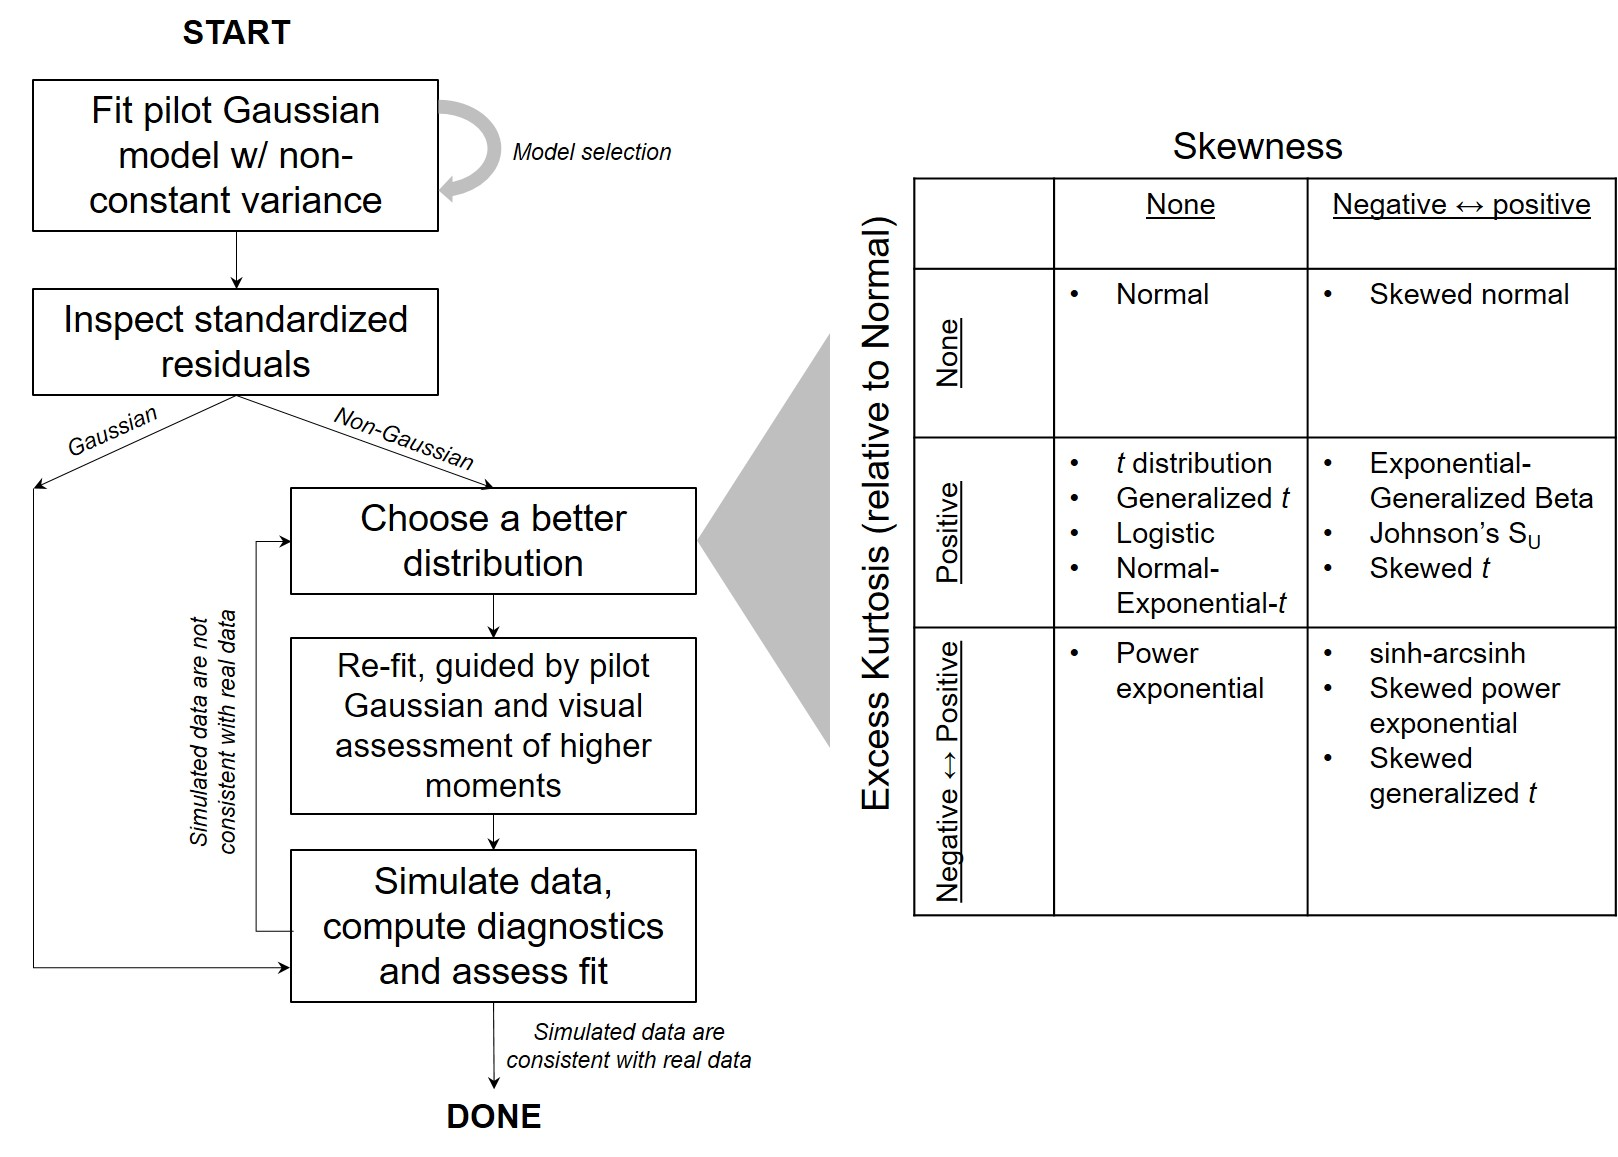
\includegraphics[width=\textwidth]{figures/workflow}
\caption{General workflow of recommendations for IPM growth modeling (left) and guide to common non-Gaussian distributions of size $x$ for $x \in \mathbb{R}$ that can accommodate different combinations of skewness and kurtosis (right). 
All of these distributions (often including multiple versions or parameterizations of each) are available in the package \textbf{gamlss.dist}, 
except for the skewed generalized $t$, which is available in the package \textbf{sgt} \citep{davis-2015}.}
%\textbf{actuar} \citep{dutang2008actuar}.
\label{fig:workflow}
\end{figure} 

\section*{How should skewness and kurtosis be measured?}
``Improvement'' of a Gaussian model will always involve scrutiny of skewness and kurtosis, so measurement of these properties warrants some attention. 
The standard measures of skewness and kurtosis (tail thickness) are based on the third and fourth central moments, respectively, of the distribution: 
\be
\mbox{Skewness} = \frac{m_3}{\sigma^3}, \quad \mbox{Excess kurtosis} = \frac{m_4}{\sigma^4}-3
\ee
where $m_k = \mathbb{E}(X - \bar{X})^k$ is the $k^{th}$ central moment of a random quantity $X$ 
and $\sigma^2$ is the variance (second central moment). 
A Gaussian distribution has zero skewness and zero excess kurtosis. 

The standard measures are easy to calculate but their use for choosing and evaluating growth models is hindered by their poor sampling properties. 
Because empirical estimates involve high powers of data values, it only takes a 
a few outliers to produce a very inaccurate estimate. 
Figure \ref{fig:NPmoments} shows a simulated example, where the underlying ``data'' are a sample of size 200 from a $t$ distribution with 8 degrees of freedom; the true skew is 0, and the true excess kurtosis is 1.5. 
The distance between the largest and smallest estimates (indicated by the dotted red vertical lines), relative to the distance between the 5th and 95th percentiles, shows the broad extent of extreme values that can occur even with a good size sample, especially for kurtosis. 

\begin{figure}[tbp]
\centering
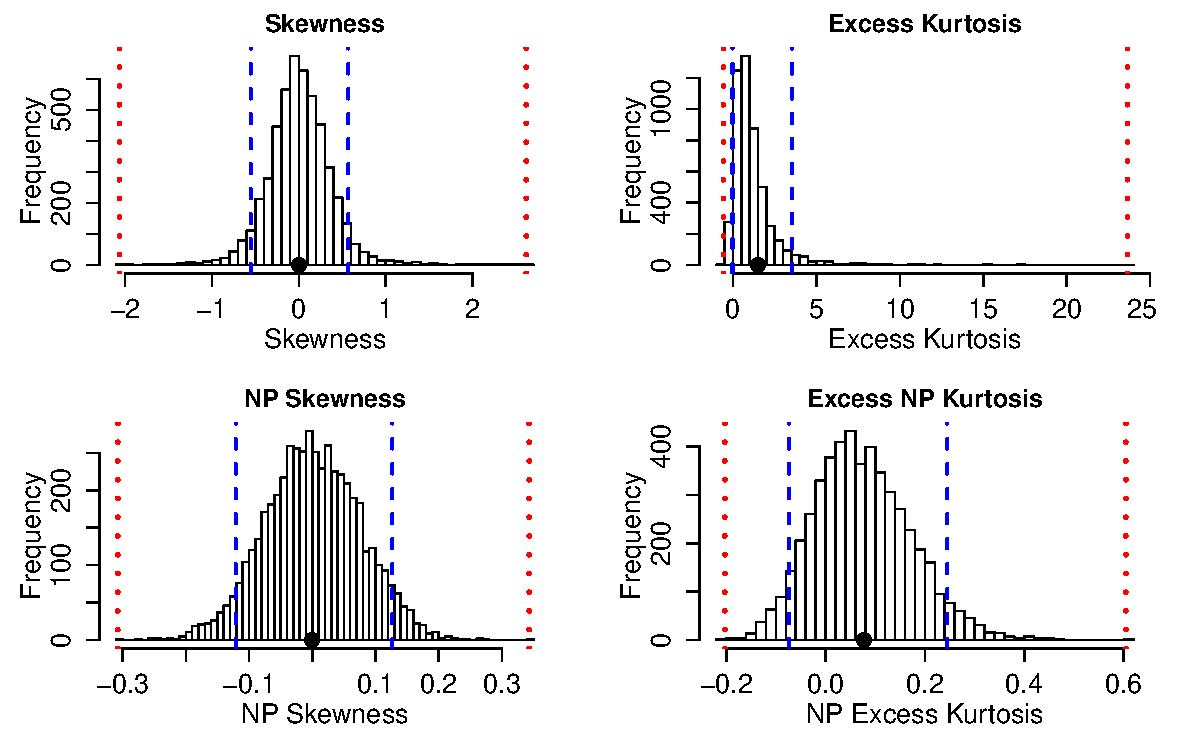
\includegraphics[width=\textwidth]{figures/NPmoments.pdf}
\caption{Histograms of skewness and kurtosis estimates using moment-based definitions, compared with the nonparametric measures. 
Histograms are based on 5000 replicate draws of a sample of 200 independent values fron a $t$ distribution with 8 degrees of freedom. 
Dotted red vertical lines mark the minimum and maximum of sample estimates, and dashed blue lines show the 5th and 95th percentiles. 
The true value is indicated by a black dot on the $x$-axis.
Figure drawn by script \texttt{NPmoments.R}}
\label{fig:NPmoments}
\end{figure} 

We therefore use ``nonparametric'' (NP) measures of skew and kurtosis that are based on quantiles and thus less sensitive to a few extreme data values. 
Let $q_\alpha$ denote the $\alpha$ quantile of a distribution or sample (e.g., $q_{0.05}$ is the 5th percentile). 
For any $0 < \alpha < 0.5$, a quantile-based measure of skewness is given by \citep{mcgillivray-1986}
\be
\mbox{NP Skewness} = \frac{q_\alpha + q_{1-\alpha} - 2 q_{0.5}}{q_{1-\alpha} - q_\alpha}.
\ee
NP Skewness is a measure of asymmetry between the tails of the distribution above and below the median. 
The size of the upper tail can be measured (for any $0 < \alpha < 0.5$) by $\tau_U = q_{1-\alpha} - q_{0.5}$; for $\alpha=0.05$ this is the difference
between the 95th percentile and the median. 
The lower tail size is $\tau_L = q_{0.5} - q_\alpha$. The definition above is equivalent to  
\be
\mbox{NP Skewness} = \frac{\tau_U - \tau_L}{(\tau_U + \tau_L)}.
\label{eqn:NPskew}
\ee
So an NP Skewness of $\pm 0.2$ says that the difference in tail sizes is 20\% of their total. 
The range of possible values is -1 to 1. Both $\alpha=0.25$ (sometimes called ``Kelly's skewness'') and $\alpha=0.1$ (``Bowley's skewness'') are common choices. 
We used $\alpha=0.1$, unless otherwise stated.  
 
An analogous quantile-based measure of kurtosis \citep{jones-etal-1994} is 
\be
\mbox{NP Kurtosis}  = \frac{q_{1-\alpha} - q_{\alpha}}{q_{0.75} - q_{0.25}}.
\label{eqn:NPkurt}
\ee
For $\alpha=0.05$, NP Kurtosis is the difference between the 95th and 5th percentiles, relative to the interquartile range. 
To facilitate interpretation, we scale NP Kurtosis relative to its value for Gaussian distribution, and subtract 1. 
We call this ``NP Excess Kurtosis''. 
The value for a Gaussian distribution is zero. 
A value of 0.2 means that the tails are (on average) 20\% heavier than those of a Gaussian with the same interquartile range, and a value of -0.2 means that the tails are (on average) 20\% lighter than a Gaussian with the same interquartile range. 
We calculate NP Kurtosis using $\alpha=0.05$ unless otherwise stated, to focus on the tail edges, but again this is somewhat arbitrary. 

Figure \ref{fig:NPmoments}C,D illustrate how, applied to exactly the same simulated samples, the non-parametric measures of skewness and kurtosis produce a smaller fraction of highly inaccurate estimates caused by a few extreme values in the sample. 
But also note that, in contrast to the moment-based measures, numerically small values of the NP measures (e.g., 0.1 or 0.2) should not be disregarded, because they are both scaled so that a value of 1 indicates extremely large departures from a Gaussian distribution. 

Quantile-based estimation of skewness and kurtosis carries the added value that quantile regression methods may be used to derive these properties of size transitions as continuous functions of initial size or expected future size. 
In the examples below, we use the \textbf{qgam} package to fit smooth additive quantile regression models, which have the flexibility to accommodate non-linear size-dependence in skewness and kurtosis. 
One risk of a gam-based approach is that fitted quantiles may be too ``wiggly'' without constraints on their complexity (in the examples below, we specify $k=4$ to constrain the dimension of the basis function). 
For the gam-averse, other quantile regression models may be equally suitable. 
For consistency with non-parametric skewness and kurtosis, we similarly use quantile-based measures of mean and variance and quantile regression to visualize these as functions of size. 
Specifically, following \cite{wan2014estimating},
\be
\mbox{NP Mean}  = \frac{q_{0.25} + q_{0.5} + q_{0.75}}{3}
\label{eqn:NPmean}
\ee
and
\be
\mbox{NP SD}  = \frac{q_{0.75} - q_{0.25}}{1.35}.
\label{eqn:NPsd}
\ee
\section{Case study: Sea fan corals, \emph{Gorgonia ventalina}}
We begin with a simple example where current size is the only predictor of future size. 
\cite{bruno-etal-2011} developed an IPM to understand the rise and fall of a fungal pathogen \emph{Aspergillus sydowii} in Caribbean sea fan corals \emph{G. ventalina}. 
The model was based on repeated observations of marked corals in permanent transects at several sites near Akumal, Mexico, recording disease status (infected/uninfected) and the area of uninfected tissue. 
The epidemic peak had passed and disease incidence was already low, so infected fans were relatively infrequent. 
We therefore limit the analysis here to uninfected individuals.
\citet{bruno-etal-2011} found statistically significant year and site effects, but as those explained a very small fraction of the variation in growth increments, they fitted a single growth model to data pooled across years and sites. 
We do the same here. 
The pooled data set consists of 358 observed size transitions. 
The data exhibited size-dependent variance in growth (change in area, $cm^2$), which \cite{bruno-etal-2011} chose to stabilize by transforming size, using the cube-root of total fan area as the size measure (fig. \ref{fig:AkumalPilot}B), and then fitting the standard model with Gaussian growth increments. 
Here we take a different approach, modeling size-dependent variance explicitly rather than trying to transform it away. 

We develop a model using natural log transformation of area. 
With initial size as the only predictor, a simple way to fit a Gaussian model with nonconstant variance is the \texttt{gam} function in \textbf{mgcv} library \citep{wood-2017} using the \texttt{gaulss} family. 
The mean and standard deviation are both fitted as smoothing spline functions of initial size, and the \texttt{predict} function returns the fitted mean and also the inverse of the fitted standard deviations with which we can compute the scaled residuals: 
\begin{lstlisting}
# XH is a data frame holding the data
# logarea.t0, .t1 denote initial and final values of log-transformed area   
fitGAU <- gam(list(logarea.t1~s(logarea.t0),~s(logarea.t0)),
              data=XH, gamma=1.4, family=gaulss())
fitted_all = predict(fitGAU,type="response"); 
fitted_sd = 1/fitted_all[,2]; 
scaledResids = residuals(fitGAU,type=''response'')/fitted_sd;  
\end{lstlisting}
Fig. \ref{fig:coral_diganostics}A shows the log-transformed data and Gaussian model. 
The mean function (solid blue curve) is visually nearly linear, but the fitted nonlinear spline is strongly favored over a linear model for the mean ($\Delta AIC \approx 9$). 
The spline for standard deviation $\sigma$ versus initial size shows that smaller individuals exhibit greater variability in future size. 

\begin{figure}[tbp]
	\centering
	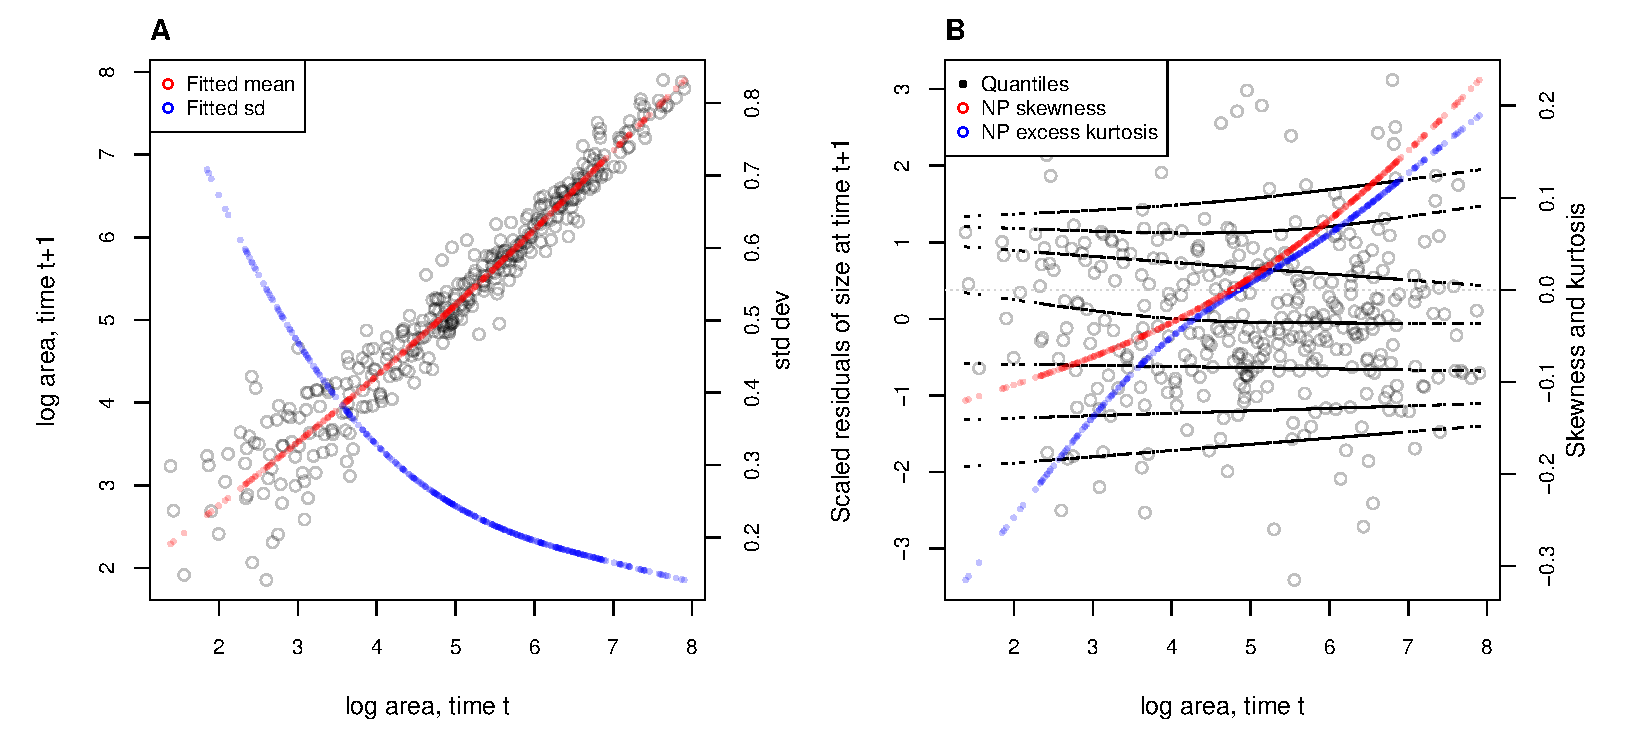
\includegraphics[width=1.0\textwidth]{figures/coral_qgam_diagnostics.pdf}
	\caption{\textbf{A}, Size transition data for sea fan corals, \emph{Gorgonia ventalina}, and fitted gam with mean (red) and standard deviation (blue) of future size conditional on current size.  \textbf{B}, Quantile regressions of scaled residuals on size and nonparametric estimates of skewness (red) and excess kurtosis (blue) derived from them. Black lines in \textbf{B} show the 5th, 10th, 25th, 50th, 75th, 90th, and 95th quantiles. Figure made by script \texttt{AkumalCorals\_qgam.R}.}
	\label{fig:coral_diganostics}
\end{figure} 

There are no blatant signs of trouble in the pilot Gaussian model, but quantile regressions on the scaled residuals, and the NP Skewness and Kurtosis metrics derived from them (Eq. \ref{eqn:NPskew} and \ref{eqn:NPkurt}), suggest deviations from normality (Fig. \ref{fig:coral_diganostics}B).
Specifically, skewness switches from negative to positive across the size distribution, with smaller corals more likely to shrink than grow and larger corals more likely to grow than shrink. 
Kurtosis also changes direction over the size distribution, with smaller initial sizes having thinner tails and larger initial sizes having fatter tails than Gaussian. 
The fitted nonparametric moments suggest that the upper and lower tails of size transition probabilities may differ by up to 20\%, and the weight of the tails may be \>20\% greater or less than Gaussian, depending on initial size -- not overwhelming deficiencies, but not trivial either. 
Are these deviations from normality severe enough to warrant a second, non-Gaussian iteration of growth modeling? 
This question may be answered by simulating data from the Gaussian model and examining whether key properties of the simulated data are consistent with those of the real data -- this is the ultimate litmus test for a growth model's adequacy and should be a standard element of IPM construction, in our opinion.
If the simulated data are not consistent with the real data, it is time to choose a better distribution (Fig. \ref{fig:workflow}). 
In this case, the negative skew at small sizes and excess kurtosis observed at large sizes are more extreme than what occurs across 100 random iterations of data simulation (Fig. \ref{fig:coral_fit}), suggesting that, for at least some parts of the size distribution, a non-Gaussian model would better capture size transitions. 

\begin{figure}[tbp]
	\centering
	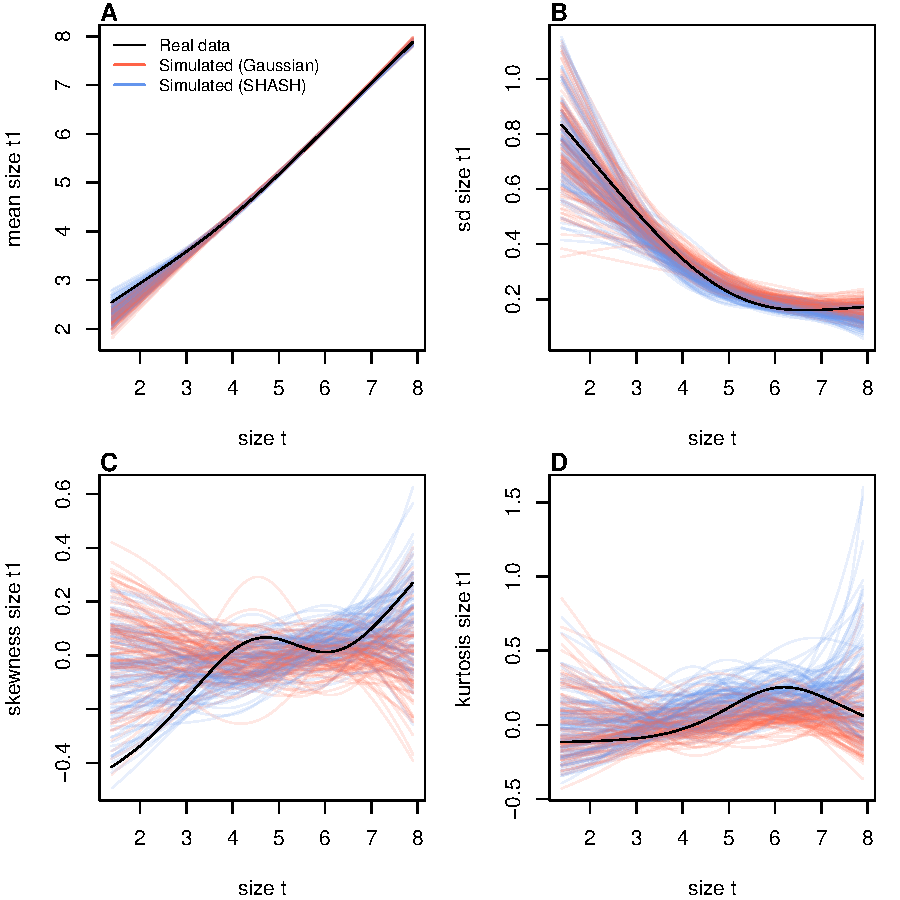
\includegraphics[width=1.0\textwidth]{figures/coral_SHASH_fit.pdf}
	\caption{Comparisons among real coral data and data simulated from Gaussian and SHASH growth models for mean, standard deviation, NP skewness, and NP kurtosis of future size conditional on current size. Figure made by script \texttt{AkumalCorals\_qgam.R}.}
	\label{fig:coral_fit}
\end{figure} 

We sought a distribution that could accommodate the properties of the scaled residuals, specifically changes in the sign of skewness and excess kurtosis across initial sizes. 
We chose the sinh-arcsinh (SHASH) distribution, a four-parameter distribution that, conveniently, is included in \textbf{mgcv}'s gam() function:
\begin{lstlisting}
	fitSHASH <- gam(list(logarea.t1 ~ s(logarea.t0,k=4), # <- location 
	~ s(logarea.t0,k=4),   # <- log-scale
	~ s(logarea.t0,k=4),   # <- skewness
	~ s(logarea.t0,k=4)), # <- log-kurtosis
	data = XH, family = shash, optimizer = "efs")
\end{lstlisting}
Data simulated from this model are more consistent with the real data than the Gaussian model: many of the 100 simulated SHASH data sets exhibited negative skew at small sizes and positive excess kurtosis at large sizes that were as strong or stronger than observed in the real data (Fig. \ref{fig:coral_fit}). 
If one cared to quantify the difference between models, the SHASH is clearly favored by AIC despite having twice as many parameters as the Gaussian ($\Delta AIC = 7.04$). 
 
What, then, have we gained by fitting a better growth model? 
Fig. \ref{fig:CoralKernelCompare}A compares the predicted distributions of subsequent size in the fitted model and Gaussian pilot models, for the median size of a new recruit (leftmost pair of curves), the median initial size (central curves), and the 95th percentile of initial size in the data (rightmost curves). 
The differences are small, and most pronounced for the smallest size, where recruits are predicted to grow slightly larger under the SHASH model than the Gaussian model. 
The direction of this difference was surprising, since the SHASH accommodates negative skew at small sizes in the data. 
However, in modeling skew appropriately, the SHASH model also gives a better prediction for mean growth at small sizes than the Gaussian model, \tom{whose mean is biased downward by negative skew (Fig. \ref{fig:coral_fit}A)}{...Contradicting the earlier assertion that parameter estimates from Gaussian models are robust to deviations from normality!}. 
Something similar happens in the standard deviation at large sizes (log size 5--7), where excess kurtosis in the data biased the SD upward (Fig. \ref{fig:coral_fit}B). 
Fig. \ref{fig:CoralKernelCompare}B shows the predicted steady-state size distributions resulting from a constant unit input of recruits. 
Again, the differences are very subtle. 
Finally, the Gaussian and SHASH growth models predict very similar mean life span (17.7 and 17.9 years, respectively).
From these outputs, there is little evidence that improved modeling of coral growth meaningfully improved biological inferences from the IPM; one could argue that it was not worth the trouble. 

\begin{figure}[tbp]
\centering
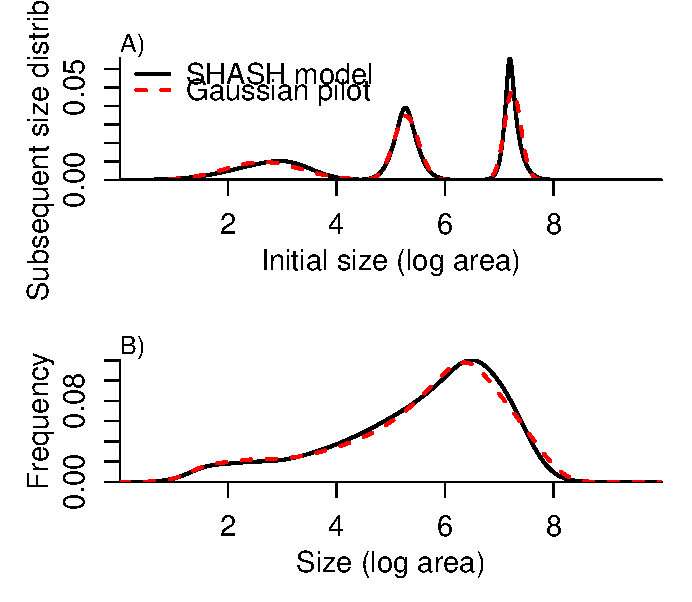
\includegraphics[width=.5\textwidth]{figures/CoralKernelCompare_v2.pdf}
\caption{Comparisons between the fitted \texttt{SEP1} growth model (solid black curves) and the Gaussian pilot model (dashed red curves)
for sea fans \emph{G. ventalina}. A) Predicted frequency distributions of size in year $t+1$ for three different values of size in 
year $t$. The leftmost pair of curves are for initial size equal to the median size of a new recruit (data from \citep{bruno-etal-2011}); 
central pair is for the median initial size of uninfected individuals; rightmost pair are for the 95th percentile initial size for uninfected
individuals. B) Steady-state size distributions resulting from a constant unit input of new recruits. As in \citet{bruno-etal-2011} we
assume that larvae are very widely dispersed, so that the number of recruits arriving at any one location is independent of the local population
abundance or structure. Size distribution of recruits was described by a kernel density estimate based on the (sadly, only $n=9$) measured sizes
of known new recruits. Figure made by script \texttt{AkumalCoralsIPMs.R}.}
\label{fig:CoralKernelCompare}
\end{figure}  

In this case study we used \texttt{gam} to fit both the Gaussian and SHASH models because that obviated model selection on functions for mean, variance, and higher moments. 
However, \texttt{gam} should be used with caution. 
Nonparametric regression models notoriously ``wag their tails'' because the ends of the fitted curve can be pulled close to the outermost data points. 
This is especially problematic for growth modeling, because data are typically sparse near the bounds of the size distribution. 
To minimize the risk of overfitting we specified the number of ``knots'' (\texttt{k=4}) and used \texttt{gamma=1.4} to overweight model degrees of freedom, as suggested by \citet[][sec. 3.2]{gu-2013}. 
But it is always important to plot the fitted splines and make sure they do not wag unrealistically. 
If they do, parametric regression may be a better choice. 

\clearpage   

\section{Case study: tree cholla cactus, \emph{Cylindriopuntia imbricata}}
The next case study, focusing on the tree cholla cactus \emph{Cylindriopuntia imbricata} at the Sevilleta Long-Term Ecological Research site in central New Mexico, adds a new feature on top of the simple size-dependent regressions in the previous study: random effects associated with temporal (year) and spatial (plot) environmental heterogeneity. 
This long-term study of cactus demography was initiated in 2004 and different subsets of the data have been analyzed in various IPM studies, all using Gaussian growth kernels  \citep{miller2009impacts,czachurademographic,compagnoni2016effect,ohm2014balancing,elderd2016quantifying}.
In fact, \citep{elderd2016quantifying} presented a Gaussian growth model fit to the cactus data as an example of a well fit growth function, based on a marginal distribution of residuals that appeared approximately Gaussian and posterior predictive checks (PPCs) of a Bayesian model that suggested consistency between the real data and data simulated from the fitted model (Fig. 4 in \citep{elderd2016quantifying}). 
While PPCs and the associated ``Bayesian P-value'' are popular diagnostic tools, they are often considered to be too conservative \citep{conn2018guide,zhang2014comparative}, failing to reject marginally bad models even though they are very effective in rejecting models that are terrible.
The choice of discrepancy function (the statistic used to compare real and simulated data) can also be limiting: in our previous work, we used a discrepancy function focused on variance (the sum of the squared residuals), so we had a built-in blind-spot for mismatches in higher moments.
In the clarity of hindsight, the PPC gave a false sense of security; the Gaussian was a poor choice all along.

The data for this new analysis include 4844 size transition observations from 929 individuals spanning 13 transition years (2004--2018) and 11 spatial replicates (three spatial blocks in years 2004--2008 and eight $30m$-by-$30m$ plots in years 2009--2018). 
The data are provided in \cite{cactusdata}.
Following previous studies, we quantified size as the natural logarithm of plant volume ($cm^3$), derived from height and width measurements. 

\begin{figure}[tbp]
	\centering
	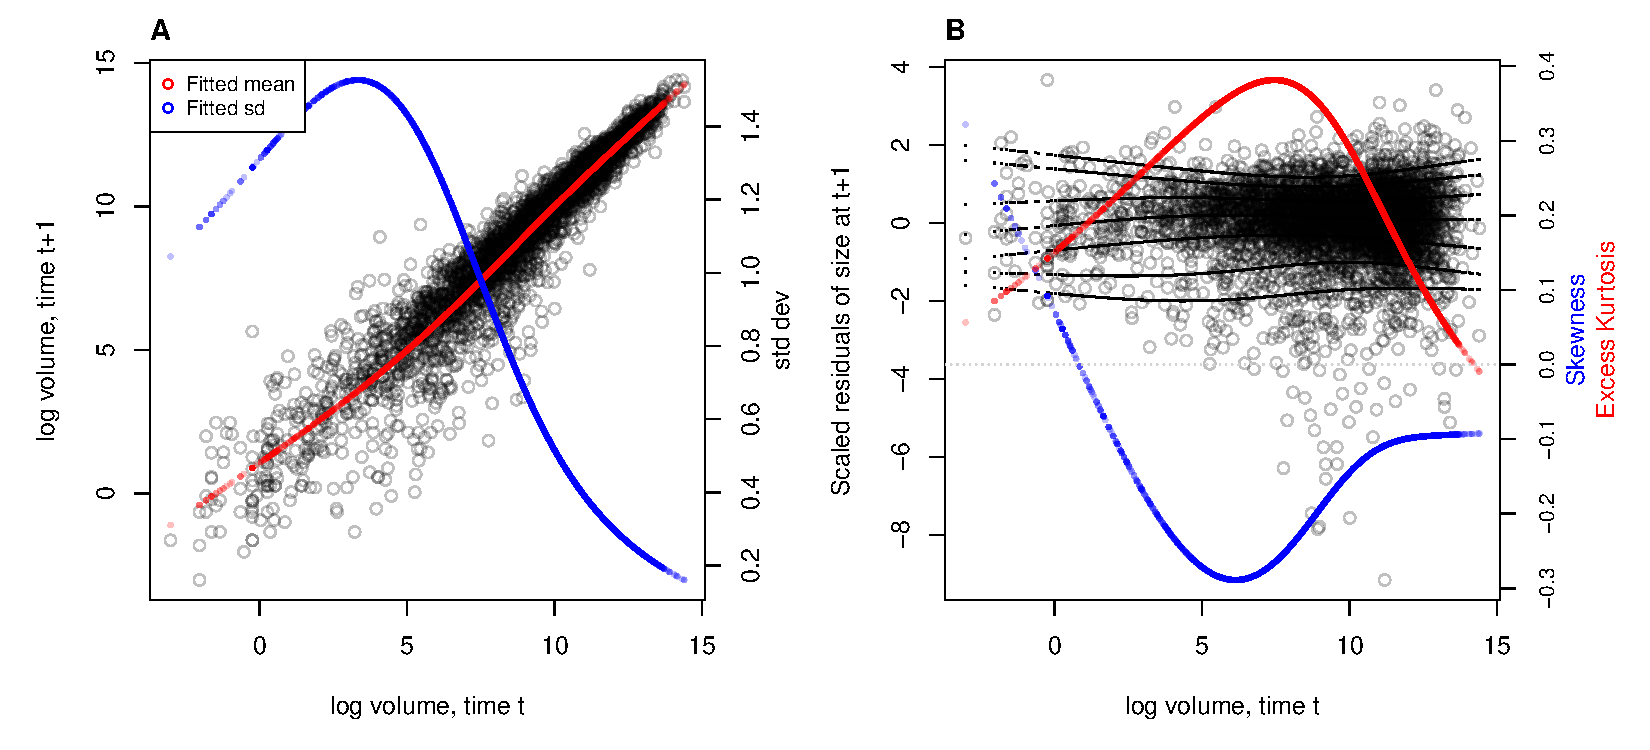
\includegraphics[width=1.0\textwidth]{figures/cactus_qgam_diagnostics.pdf}
	\caption{\textbf{A}, Size transition data for tree cholla cacti, \emph{Cylindriopuntia imbricata}, and fitted gam with mean (red) and standard deviation (blue) of future size conditional on current size.  \textbf{B}, Quantile regressions of scaled residuals on size and nonparametric estimates of skewness (red) and excess kurtosis (blue) derived from them. Black lines in \textbf{B} show the 5th, 10th, 25th, 50th, 75th, 90th, and 95th quantiles. Figure made by script \texttt{cactus\_growth\_modeling\_qgam.R}.}
	\label{fig:cactus_diganostics}
\end{figure} 


We begin the growth modeling workflow, as above, with a generalized additive model with the mean and standard deviation of size in year $t+1$ modeled as function of size in year $t$, with random intercepts for year and plot and assuming normally distributed residuals (\texttt{family=gaulss()}). 
The standardized residuals, accounting for size-dependent residual variance (Fig. \ref{fig:cactus_diganostics}A), show clear signals of negative skew and positive excess kurtosis across most of the size distribution but strongest in the middle of the size distribution (Fig. \ref{fig:cactus_diganostics}B). 

To better capture size transitions, we need a distribution with negative skew and positive excess kurtosis, but both of which may be negligible at some sizes.
We first tried Johnson's $S_{U}$ and then the skewed $t$ distributions, both of which are limited to positive excess kurtosis.
Both distributions provided some improvement over the Gaussian, but were not happy with the fit of either. 
Iterating through the workflow (Fig. \ref{fig:workflow}), we arrived, again, at the SHASH distribution, which is more flexible than either the JSU or skewed $t$, capable of capturing a greater range of kurtosis for a given amount of skew, and vice versa (Steve's NPSkewKurtosisRanges.pdf). 
Furthermore, fitting the SHASH as a generalized additive model with \textbf{mgcv} allowed for flexible, non-monotonic size-dependence in skewness and kurtosis without the need for model selection on specific size-dependent functions; through iterations of trial and error, we found this flexibility was necessary to generate simulated data that compared favorably to the real data. 
The other distributions that we tried are not available as \textbf{mgcv} families, so we fit these with custom maximum likelihood functions, an approach we illustrate in the next case study.
The final growth model was similar to the SHASH gam in the coral case study, but with random intercepts for the location parameter, representing spatial and temporal heterogeneity:
\begin{lstlisting}
fit_shash <- gam(list(logvol_t1 ~ s(logvol_t,k=4) + 
				s(plot,bs="re") + s(year_t,bs="re"), # <- model for location 
				~ s(logvol_t,k=4),   # <- model for log-scale
				~ s(logvol_t,k=4),   # <- model for skewness
				~ s(logvol_t,k=4)), # <- model for log-kurtosis
			data = CYIM_grow, 
			family = shash,  
			optimizer = "efs")
\end{lstlisting}

The final SHASH model provided good correspondence between simulated and real data, and provided more compelling improvement over the Gaussian model than we saw in the coral case study (Fig. \ref{fig:cactus_fit}). 
The SHASH model over-estimated negative skew at some sizes relative to the signal of skewness in the data (Fig. \ref{fig:cactus_fit}C), but the nature of size-dependent skew in the data is not very biologically plausible and may instead be driven by the tail-wagging tendency of gams. 
As in the coral case study, we see that correctly modeling skewness and kurtosis improved estimation of the mean and standard deviation (Fig. \ref{fig:cactus_fit}A,B), yielding a growth model that is clearly truer to the data than the pilot Gaussian fit. 

\begin{figure}[tbp]
	\centering
	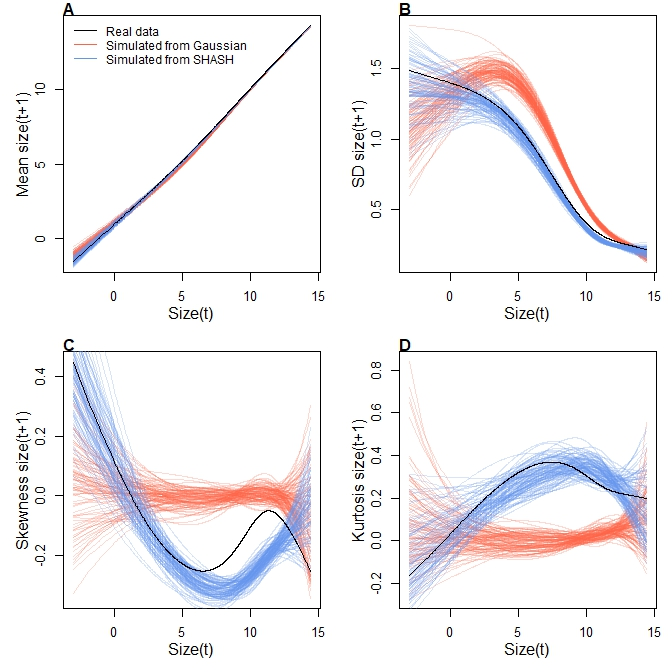
\includegraphics[width=1.0\textwidth]{figures/cactus_SHASH_fit.pdf}
	\caption{Comparisons among real cactus data and data simulated from Gaussian and SHASH growth models for mean, standard deviation, NP skewness, and NP kurtosis of future size conditional on current size. Figure made by script \texttt{cactus\_growth\_modeling\_qgam.R}.}
	\label{fig:cactus_fit}
\end{figure} 

We explored how improved growth modeling influenced IPM results, leveraging the plot and year structure of the study design to quantify spatial and temporal variance in fitness.
We used the fitted random effects from the vital rate models to estimate the asymptotic growth rate for each year ($\lambda_t$), centered on the average plot, and for each plot ($\lambda_p$), centered on the average year.
This allowed us to quantify demographic variance associated with temporal and spatial heterogeneity. 
We found that the Gaussian growth model tended to over-estimate $\lambda_t$, particularly in the harshest years (Fig. \ref{fig:cactus_lambda}A), and thus under-estimated temporal variance in fitness ($Var(\lambda_{t(Gaussian)})=0.0018$, $Var(\lambda_{t(SHASH)})=0.0023$). 
The opposite was true for plot-to-plot variation (Fig. \ref{fig:cactus_lambda}B), where the Gaussian model under-estimated $\lambda_p$ and over-estimated spatial variance in fitness ($Var(\lambda_{p(Gaussian)})=0.00015$, $Var(\lambda_{p(SHASH)})=0.000088$). 
Across both growth models, fluctuations in fitness were stronger through time than across space. 
The difference in temporal variance would suggest that Gaussian growth modeling would lead to over-estimation of the stochastic growth rate $\lambda_S$, since temporal variance has a negative influence on $\lambda_S$.
However, this was not the case: stochastic IPMs based on Gaussian and SHASH growth models had nearly identical stochastic growth rates ($\lambda_S(Gaussian)=0.9906$, $\lambda_S(Gaussian)=0.9909$). 
This is likely because temporal fluctuations in vital rates, which is where the SHASH growth model would make a difference, have a weaker influence on $\lambda_S$ than the temporal fluctuations in size structure that they generate \citep{ellis2013role,compagnoni2016effect}. 
Thus, depending on the target of one's analysis, modeling non-Gaussian size transitions with a Gaussian growth model could bias results in either direction, or make no difference at all. 

%We did so using the `kernel selection' method, sampling transition kernels constructed with year- and plot-specific random effects, rather than sampling year and plot deviates from their fitted variances; the kernel selection approach has the advantage of retaining any spatial or temporal correlation in the vital rates. 

\begin{figure}[tbp]
	\centering
	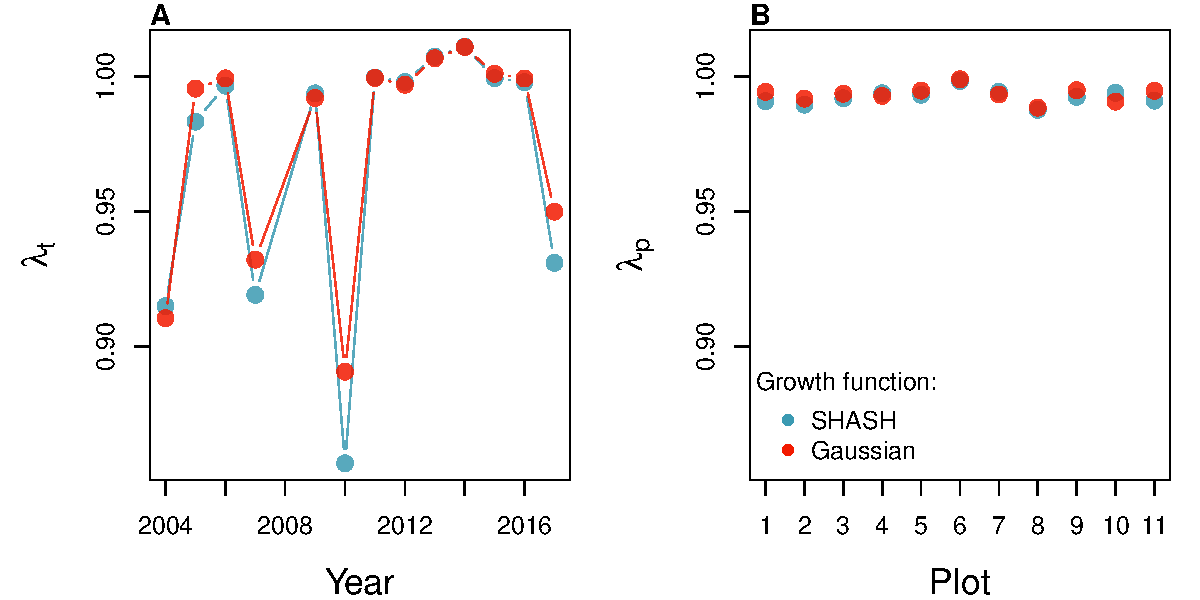
\includegraphics[width=1.0\textwidth]{figures/cactus_lambda_years_plots.pdf}
	\caption{Temporal (\textbf{A}) and spatial (\textbf{B}) heterogeneity in fitness for the tree cholla cactus (\textit{Cylindriopuntia imbricata}) predicted by IPMs using Gaussian or SHASH growth models. Figure made by script \texttt{cactus\_growth\_modeling\_qgam.R}.}
	\label{fig:cactus_lambda}
\end{figure} 


\section{Case study: creosotebush, \emph{Larrea tridentata}}
Our next case study comes from our studies of the woody shrub creosotebush (\emph{Larrea tridentata}) at the Sevilleta Long-Term Ecological Research (LTER) site in central New Mexico, US. 
At this site as elsewhere in the Southwest US, creosotebush is encroaching into desert grassland habitats.
The data described here were collected along transects spanning grass-shrub ecotones to understand patterns of density dependence in creosotebush demography.
Specifically, we asked whether fitness is maximized approaching zero density at the leading edge of the expansion front (consistent with `pulled' expansion), or whether there is a demographic advantage for shrubs at higher density due to positive feedbacks expected for ecosystem engineers (leading to `pushed' expansion). 
Our published study \citep{drees2023demography} used a spatial integral projection model (SIPM) to predict the speed of shrub encroachment, assuming normally-distributed size transitions. 
Here we step through our suggested workflow to ask whether a non-Gaussian model would have been more faithful to the data, and how such an improvement would influence predictions for the speed of encroachment.
We use this case study to illustrate several new elements and challenges, including modeling skewness and kurtosis as functions of expected future size (instead of initial size) and using distributions that are not currently available as \textbf{mgcv} families.
In fact, to diversify our use of software and illustrate alternatives, we do not use gam's for any element of this case study.

Growth data come from 522 shrubs censused longitudinally over four years (2013-2017). 
Census individuals occurred along 12 replicate transects (200 to 600 m in length) that spanned gradients of shrub density along shrub-grass ecotones. 
Size was measured as volume of an elliptical cone based on height and width measurements; the size variable of the IPM was the natural logarithm of volume ($cm^3$). 
For each census individual, we recorded the size and density of all conspecifics within the five-meter transect ``window'' in which it occurred, and took the sum of all sizes within the window as a measure of local density. 
The data are available in \cite{shrubdata}. 

As an initial Gaussian approach, we first fit a set of candidate generalized linear mixed models, including transect as a random effect, that represented competing hypotheses for how size, density, and their interaction influence growth. 
Specifically, we fit five candidate Gaussian models that included fixed effects of initial size only (model 1), size and density (model 2), and size, density, and their interaction (model 3), allowing for shrubs of different sizes to have different growth responses to local density. 
Models 4 and 5 mirrored models 2 and 3 but included second-order terms for density, allowing for the possibility of non-monotonic density dependence. 
As in \citep{drees2023demography} we pooled data across three transition years. 
Initial AIC rankings of these pilot models favor model 4 slightly over model 5 ($\Delta AIC = 0.8$) and significantly over all other models ($\Delta AIC > 2$). 
However, these models were fit assuming constant variance, and inspection of the residuals of the best model indicate this is not a safe assumption. 

Unlike our previous case studies, here we have multiple fixed effects that may influence the variance of future size. 
In cases such as this, we recommend modeling variance as a function of expected future size rather than initial size, as we did with the corals and cacti. 
The expected (or ``fitted'') values reflect the combined influence of all fixed and random effects, and therefore implictly account for multiple sources of variation in the variance. 
While there are several convenient software packages for simultaneously modeling Gaussian mean and variance as functions of independent variables (\textbf{mgcv} for additive models as we saw above, \textbf{nmle} for linear models), \tom{modeling variance as a function of the mean is trickier because they cannot easily be fit simultaneously}{After I wrote this I discovered that nlme can fit residual variance as a function of fitted(.).}. 
Here we us an iterative re-weighting approach -- which is not elegant, but it works. 
For Gaussian models, weights $w_{i}$ can be used to indicate that the observations $y_{i}$ vary in their dispersion around the mean. 
In general, the iterative steps are: 
\begin{enumerate}
	\item Fit the expected value and normally-distributed residuals with constant variance:
	$$y_{i} = \mu_{i} + \epsilon_{i}$$
	$$\epsilon_{i} \sim N(0,\sigma)$$
	\item Fit the standard deviation of the residuals as a function of the expected value. Weights are derived as the inverse of the fitted variance:
	$$\epsilon_{i} \sim N(0,f(\mu_{i}))$$
	$$w_{i}=1/{f(\mu_{i})^2}$$
	\item Re-fit the observation model, weighting the residual variance according to step 2:
	$$y_{i} = \mu_{i} + \epsilon_{i}$$
	$$\epsilon_{i} \sim N(0,\sigma \times \sqrt{w_{i}})$$	
\end{enumerate}
We iterated steps 2 and 3 until the weights did not change. 
In step 2, we modeled the standard deviation as a simple linear function of the expected value ($log(f(\mu_{i}))=\beta_{0}+\beta_{1}*\mu_{i}$) but other functions are possible, as is model selection among them. 
We did this for all candidate models and, for fair AIC comparison, we re-fit all candidate models with the same weights, estimated from the top model. 
The updated model selection continued to favor model 4, but now with a stronger improvement over the next-best model ($\Delta AIC = 3.0$). 

\begin{figure}[tbp]
	\centering
	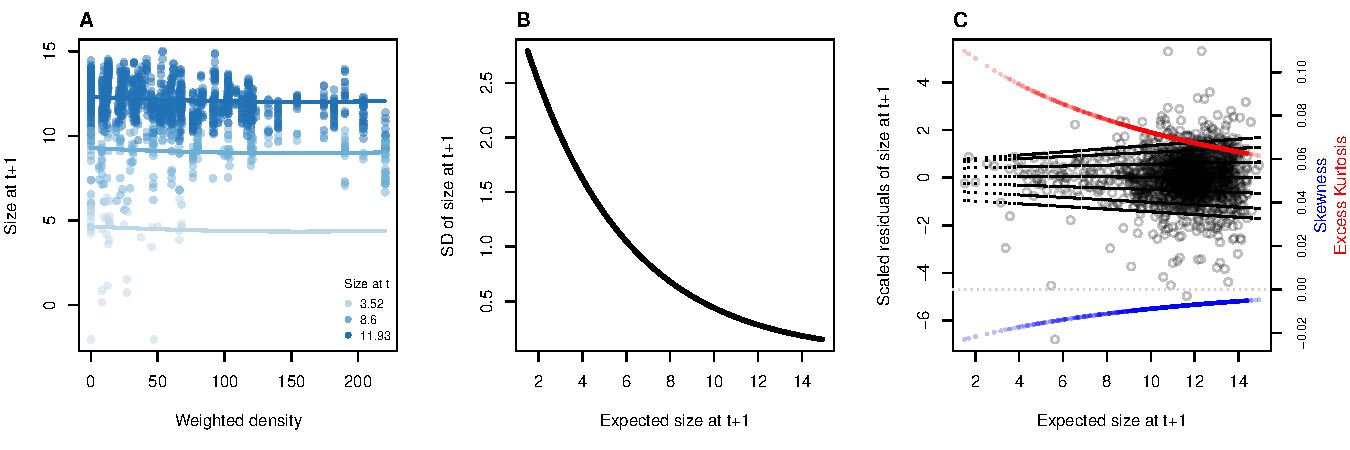
\includegraphics[width=1.0\textwidth]{figures/creosote_diagnostics.pdf}
	\caption{\textbf{A}, Creosotebush size transition data with repsect to initial size (colors) and local weighted density (sum of sizes of all plants within a five-meter transect window). Size is quantified as the natural logarithm of plant volume ($cm^3$). \textbf{B}, Standard deviation of size at time $t+1$ as a function of expected size at $t+1$ (the fitted values), estimated by iterative re-weighting. \textbf{C}, Quantile regressions of scaled residuals on size and nonparametric estimates of skewness (blue) and excess kurtosis (red) derived from them. Black lines in \textbf{C} show the 5th, 10th, 25th, 50th, 75th, 90th, and 95th quantiles. Figure made by script \texttt{creosote\_growth\_modeling\_qgam.R}.}
	\label{fig:creosote_diganostics}
\end{figure} 

The resulting Gaussian growth model predicts strong initial size-dependence and weak and slightly nonlinear (but monotonic) negative density dependence (Fig. \ref{fig:creosote_diganostics}A). 
The model accounts for non-constant variance through the fitted weights, which indicate greater dispersion for smaller values of expected size ($\beta_{1}=-0.21$; Fig. \ref{fig:creosote_diganostics}B). 
Quantiles of the standardized residuals indicate weak negative skew (difference in tail size is 1--2\% of their total) and positive excess kurtosis, especially at smaller expected sizes (tails are 6--10\% fatter than Gaussian) (Fig. \ref{fig:creosote_diganostics}C). \tom{}{Note that there is still a variance trend in the standardized residuals--rather unsatisfying! I have been through this backwards and forwards and my take is that this is a product of the sample size imbalance between small and large plants. The quantile regression is doing its best.}
As a candidate for improvement, we turned to the Johnson's $S_{U}$ (JSU) distribution, a four-parameter, leptokurtic distribution capable of skew in either direction. 
We used a parameterization of the JSU for which location parameter $\mu$ is the mean and scale parameter $\sigma$ is the standard deviation \citep{rigby2019distributions}. 

Like many of the non-Gaussian candidates that we suggest (Fig. \ref{fig:workflow}), the JSU distribution is not presently available as a family option for linear mixed models in any software package, to our knowledge. 
However, this need not be a barrier to using it for growth modeling. 
We fit a custom maximum likelihood model that borrows the mean and standard deviation of best Gaussian model and limits estimation of free parameters to those that control the JSU's skewness and kurtosis -- effectively modeling the standardized residuals rather than sizes. 
Here is what such a hybrid likelihood model looks like in practice:
\begin{lstlisting}
## log_volume_t1 are the size obervations
## GAU_fitted are the expected values of the best Gaussian model
## pars is a vector of free parameters to be estimated
JSULogLik=function(pars){
	dJSU(x=log_volume_t1, 
	mu=GAU_fitted,
	sigma=exp(GAU_sd_coef[1]+GAU_sd_coef[2]*GAU_fitted),
	nu = pars[1]+pars[2]*GAU_fitted,
	tau = exp(pars[3]+pars[4]*GAU_fitted), log=TRUE)
}
\end{lstlisting}
The mean of the JSU is set to that of the best Gaussian model (\verb|GAU_fitted|) and the standard deviation is a function of the mean according to the coefficients (\verb|GAU_sd_coef|) estimated through iterative re-weighting. 
Based on diagnostics of the standardized residuals (Fig. \ref{fig:creosote_diganostics}), JSU parameters that control skewness and kurtosis are defined as linear functions of the mean, and it is these coefficients that are estimated by maximum likelihood. 
Here we are relying on the robustness of Gaussian linear models to deviations from normality . 
If one is skeptical of this approach, it is possible, as an alternative, to simultaneously re-fit all parameters of the JSU in a maximum likelihood framework. 
However, incorporating random effects into a custom likelihood model is non-trivial (we provide guidance on one way to do this, using the ``shrinkage'' approach, in Appendix XX). 
Therefore a key advantage of the hybrid approach is convenient retention of the fitted random effects and associated variance components, which get shuttled from the Gaussian model into the non-Gaussian model without any fuss (it was critical that we used a parameterization of the JSU for which \verb|mu| is the mean and \verb|sigma| is the standard deviation). 
And, if this approach does not ``work'' (i.e., deviations from normality biased the fitted values of the Gaussian model) one would quickly find out through the simulation step of the workflow. 
In this case, the hybrid JSU model performed well, generating simulated data that aligned with the real data better than the best Gaussian model, particularly in \tom{standard deviation}{I am a little mystified as to why the JSU is so much better. It is literally the same SD in both distributions.} and kurtosis (Fig. \ref{fig:creosote_JSU}). 
Note that in Fig. \ref{fig:creosote_JSU} we are plotting moments of the future size distribution with respect to initial size; this distribution is also conditional on density but initial size is by far the stronger predictor of future size, so we chose this visualization. 

\begin{figure}[tbp]
	\centering
	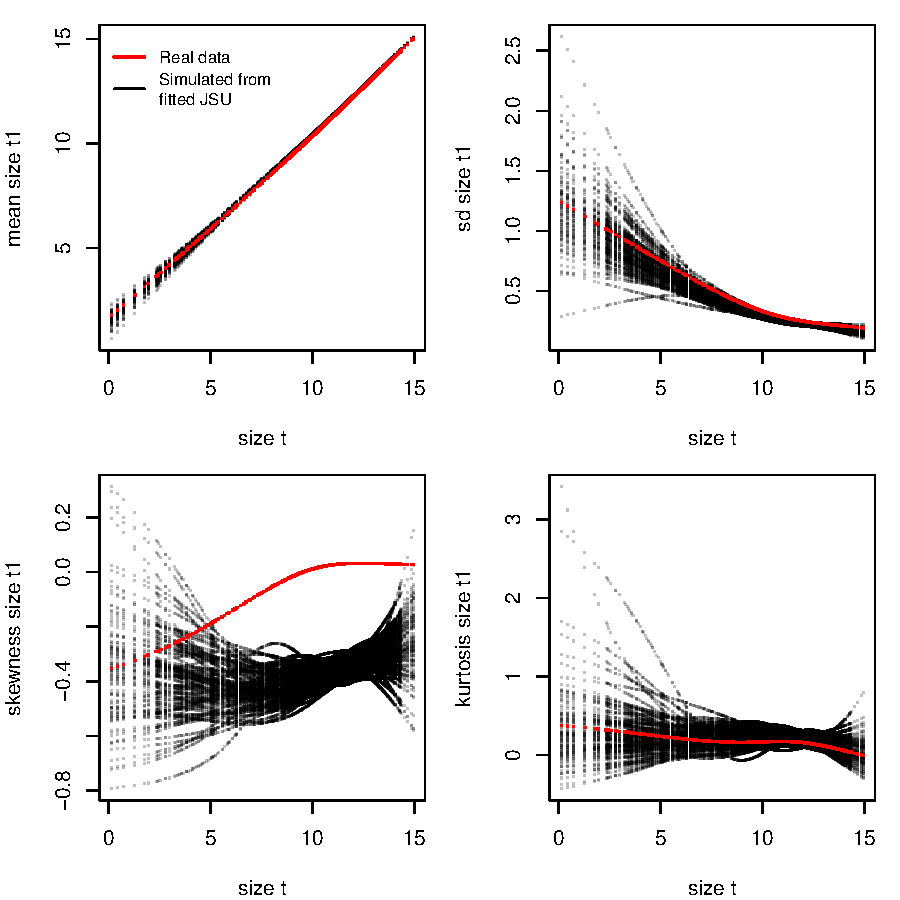
\includegraphics[width=1.0\textwidth]{figures/creosote_JSU_fit.pdf}
	\caption{Comparisons between real creosotebush data and data simulated from Gaussian and JSU growth models for mean, standard deviation, NP skewness, and NP kurtosis of future size conditional on current size. Figure made by script \texttt{creosote\_growth\_modeling\_qgam.R}.}
	\label{fig:creosote_JSU}
\end{figure} 

The improvement of the JSU over the Gaussian growth model, while visually satisfying, had virtually no influence on SIPM results. 
Models using Gaussian or JSU growth kernels had nearly identical, monotonic decreases in $\lambda$ with increasing local density, and nearly identical wave velocities (Fig. \ref{fig:creosote_lambda_cstar}). 
This species has very low mortality risk once established (mean remaining life expectancy of a median-sized shrub is 24,408 years) and its population growth and wave expansion are limited by very low seedling recruitment (\citep{drees2023demography}). 
Weak size-dependence in survival likely explains why the improvement in growth modeling had little influence on SIPM predictions. 

\begin{figure}[tbp]
	\centering
	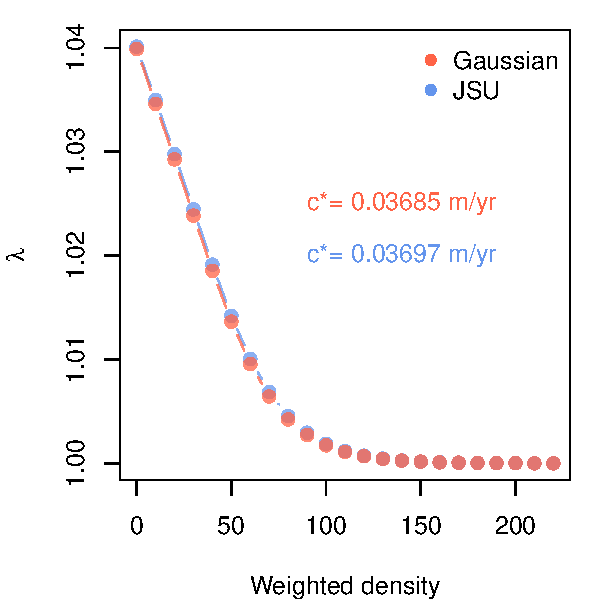
\includegraphics[width=0.5\textwidth]{figures/creosote_DD_lambda.pdf}
	\caption{Density dependence in fitness ($\lambda$) and asymptotic velocity of the creosote encroachment wave (c*) for Gaussian and JSU growth kernels. Weighted density is the sum of sizes ($log(cm^3)$) of all conspecifics within a five-meter transect ``window''. Figure made by script \texttt{creosote\_growth\_modeling\_qgam.R}.}
	\label{fig:creosote_lambda_cstar}
\end{figure}

\section{Case study: lady orchid, \emph{Orchis purpurea}}
Our final case study examines selection on life history strategies in the lady orchid \textit{Orchis purpurea}. 
In a prior study, Miller et al. \citeyear{miller2012evolutionary} contrasted the growth trajectories from year $t$ to $t+1$ for plants that did or did not flower in year $t$, as a way to quantify costs of reproduction. 
The different growth kernels were then used in an IPM to quantify evolutionarily stable life history strategies: the optimal flowering size that balances benefits of flowering at larger sizes against the risk of dying before reaching those sizes. 
The original study assumed a Gaussian distribution of size transitions and allowed for non-constant variance with respect to initial size. 
Here we re-visit that analysis applying our growth modeling workflow to derive improved growth kernels for flowering and non-flowering orchids. 

The data, originated by Dr. Hans Jacquemyn and used here with permission, come from 368 plants in a Belgian population that was censused annually from 2003 through 2011 (for this reanalysis we are using data only from the ``light'' habitat). 
Size was measured as leaf area ($cm^3$) summed over all leaves, and we analyzed the natural logarithm of total leaf area as the size variable of the IPM. 

As a pilot Gaussian approach, we fit six candidate models in which the mean was a function of initial size only, additive effects of initial size and flowering status, and interaction between size and flowering, and the standard deviation was a function of size only (models 1-3) or size and flowering status (models 4-6). 
All models included a random intercept for year. 
As another variation on software and an alternative to two-step fitting or iterative re-weighting, here we use \verb|nmle::lme()|, which can simultaneously fit linear predictors for mean and variance. 
For example, model 1 was:
\begin{lstlisting}
orchid_GAU[[1]]<-lme(log_area_t1~log_area_t,
	weights=varExp(form=~log_area_t),
	random=~1|begin.year,data=orchid_grow,method="ML")
\end{lstlisting}
Model 3 (size $\times$ flowering) was strongly favored, consistent with prior results that non-flowering plants have a growth advantage over flowering plants. 
Growth variance declined with initial size for both reproductive classes (Fig. \ref{fig:orchid_diagnostics}A-B) and skewness and kurtosis of the standardized residuals indicate strong deviations from normality (Fig. \ref{fig:orchid_diagnostics}C-D). 
For most sizes, left skew and excess kurtosis were more severe for non-reproductive plants, with tail imbalance ca. 10\% of their total and tail weights 10--20\% fatter than Gaussian. 

\begin{figure}[tbp]
	\centering
	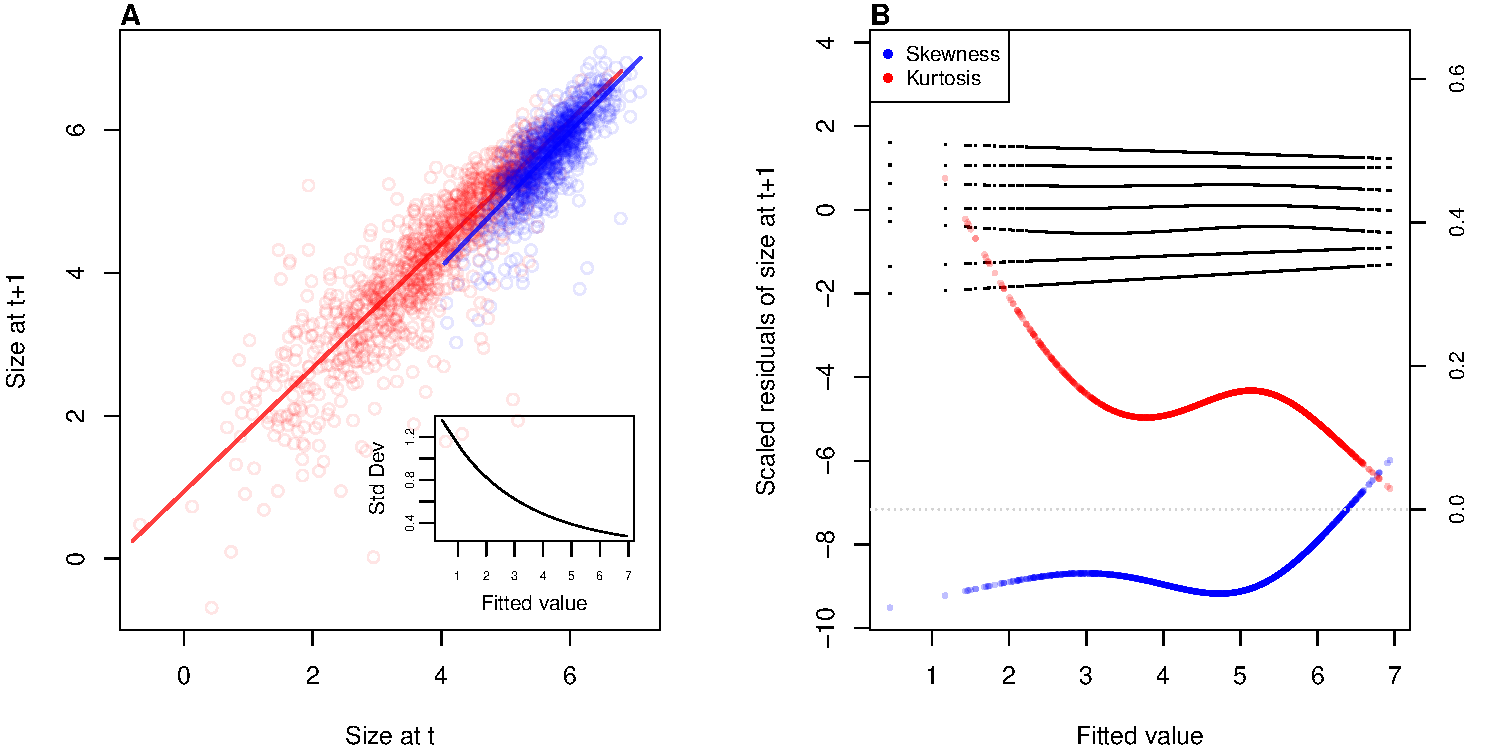
\includegraphics[width=1.0\textwidth]{figures/orchid_diagnostics.pdf}
	\caption{}
	\label{fig:orchid_diagnostics}
\end{figure} 

As improvements, we explored the skewed $t$ and Johnson's SU distributions, both leptokurtic distributions with flexible skewness. 
We were happier with the skewed $t$, which we fit in a similar way as we fit the JSU to the creosote data, setting the mean and standard deviation to the Gaussian fits and estimating free parameters controlling skewness and kurtosis:
\begin{lstlisting}
## log_area_t1 and log_area_t are the size obervations
## flowering indicates reproductive status at time t (0 or 1)
## GAU_fitted and GAU_sd are mean and standard deviation from lme
## pars is a vector of free parameters to be estimated
SSTLogLik=function(pars){
	dSST(x=log_area_t1, 
	mu=GAU_fitted,
	sigma=GAU_sd,
	nu = exp(pars[1] + pars[2]*log_area_t + pars[3]*as.logical(flowering) + pars[4]*log_area_t*as.logical(flowering)),
	tau = exp(pars[5] + pars[6]*log_area_t + pars[7]*as.logical(flowering) + pars[8]*log_area_t*as.logical(flowering))+2, 
	log=TRUE)
}
\end{lstlisting}
\verb|gamlss.dist:dSST| is a parameterization of the skewed $t$ in which \verb|mu| and \verb|sigma| are the mean and standard deviation, respectively. 
Based on diagnostics of the standardized residuals (Fig. \ref{fig:orchid_diagnostics}) we allowed \verb|nu| and \verb|tau| to vary by size and differ between flowering and non-flowering plants (note that the \verb|tau| parameter uses a $log(x-2)$ link function). 
Size transition data simulated from this model corresponded favorably to the real data, much better than the pilot Gaussian model, including improvements in the \tom{standard deviation}{Again, the improvement here is suprising to me and I am unsure what to say about it.}, skewness, and kurtosis of future size (Fig. \ref{fig:orchid_SST_fit}). 

\begin{figure}[tbp]
	\centering
	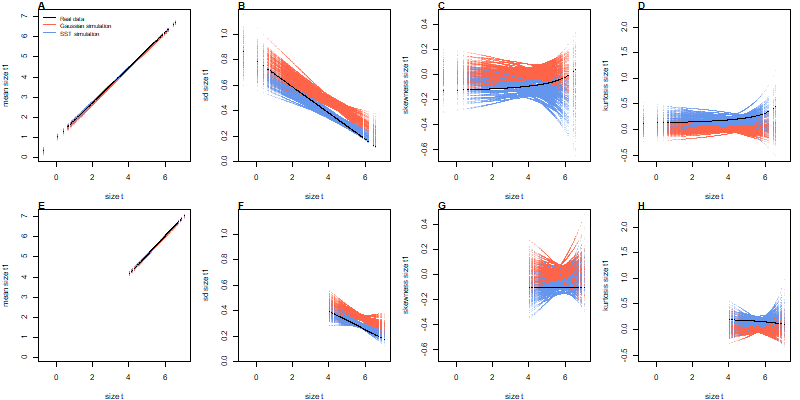
\includegraphics[width=1.0\textwidth]{figures/orchid_SST_fit.pdf}
	\caption{Comparisons between real orchid data and data simulated from Gaussian and skewed $t$ growth models for mean, standard deviation, NP skewness, and NP kurtosis of future size conditional on current size. Top row (\textbf{A}-\textbf{D}) shows plants that were vegetative at the start of the transition year and bottom row (\textbf{E}-\textbf{H}) shows plants that were flowering at the start of the transition year. Figure made by script \texttt{orchid\_growth\_modeling\_rq.R}.}
	\label{fig:orchid_SST_fit}
\end{figure} 

Finally, we used the improved growth model to revisit key results of the original study. 
Miller et al. (\citeyear{miller2012evolutionary}) used the orchid IPM to estimate the evolutionarily stable strategy (ESS) as the mean size at flowering that maximizes lifetime reproductive success ($R_0$), given the constraint that flowering when small reduces growth and thus elevates mortality risk. 
Repeating that analysis here, we found that improved growth modeling has virtually no influence on predictions for optimal life history strategies (Fig. \ref{fig:orchid_ESS}).
ESS flowering sizes were nearly identical between IPMs with Gaussian vs skewed $t$ growth models, and both aligned well with the observed mean flowering size (dashed vertical line in Fig. \ref{fig:orchid_ESS}A). 
Extending beyond the original study, we also explored expected remaining lifespan for different ages and sizes (R package \textbf{Rage} \citep{jones2022rcompadre}). 
Gaussian and skewed $t$ growth models predicted nearly identical mean remaining lifespans across the stage and size distribution (Fig. \ref{fig:orchid_ESS}B).
\tom{However, the skewed $t$ model predicted consistently greater variance in remaining lifespan, nearly 10\% greater at some sizes.}{Do not believe this result! I have left it here as a placeholder because I would like to do this correctly. But I think there are problems with Rage's life\_expect\_var() function. The predicted variance declines linearly with matrix dimension.} 
Thus, as we have seen in other case studies, the practical consequences of improved growth modeling depend on what one aims to learn from the IPM. 

\begin{figure}[tbp]
	\centering
	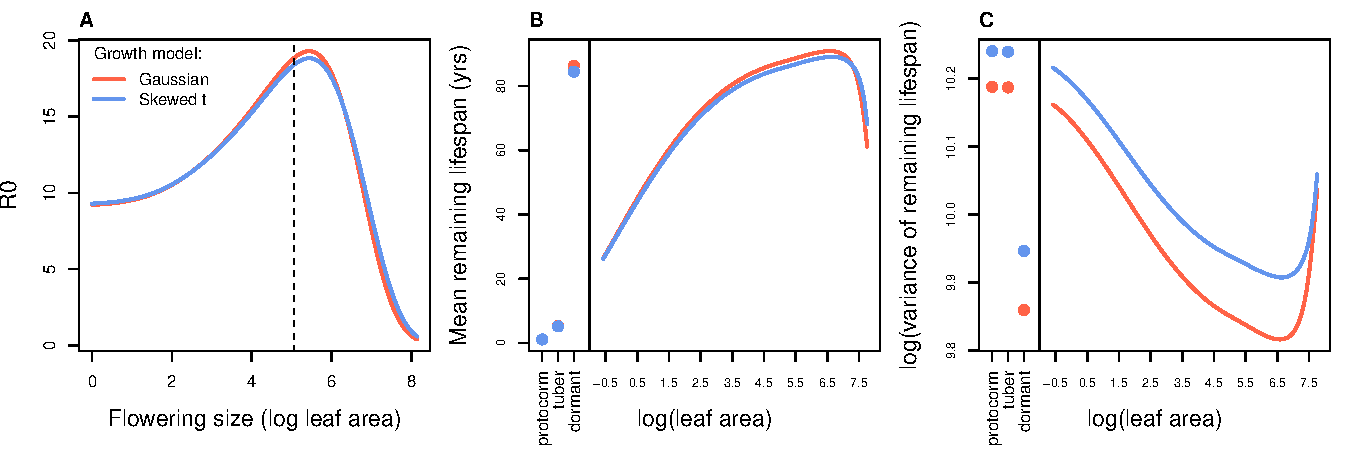
\includegraphics[width=1.0\textwidth]{figures/orchis_life_history.pdf}
	\caption{Orchid life history results from IPMs using Gaussian or skewed $t$ growth models. \textbf{A}, Lifetime reproductive success ($R_0$) as a function of mean size of flowering. Dashed vertical line shows the observed mean flowering size. \textbf{B-C}, Mean and variance of remaining lifespan as a function of size or stage. The orchid IPM includes three discrete below-ground stages (protocorm, tuber, and dormant plant) in addition to continuous size of above-ground plants.}
	\label{fig:orchid_ESS}
\end{figure} 

\section{Discussion}
Much of the appeal of integral projection models has stemmed from their embrace of continuous size structure through reliance on regression-based approaches, and the potentially complex fixed- and random-effect structures that these approaches allow. 
Using familiar statistical tools and with relatively few parameters to estimate, IPM users can incorporate important sources of variation in demography and interrogate their influence on ecological and evolutionary dynamics. 
With this opportunity comes the burden of getting it right: IPMs are good models of the populations they are intended represent only insofar as the statistical models provide good fits to the underlying data. 
The growth sub-model is the trickiest part of ``getting it right'' because it defines a distribution of future size conditional on current size. 
Distributions have many properties -- ``moments'' -- and a good growth model should recapitulate the properties of real size transitions. 
The default assumption of normally distributed size transitions, employed overwhelmingly across 20+ years of IPM studies, is an arbitrary historical precedent. 
In four case studies (chosen simply because we had the data at our fingertips) and, we suspect, more broadly, skewness and excess kurtosis were common features of size transition data: shrinking was more common than growing, and large changes in size were more common than a Gaussian model would predict. 
Our most important message is that the standard assumption of normally-distributed size transitions should be abandoned and a more inquisitive process of growth modeling should take its place. 

We have attempted to lay out a general workflow for what that process should look like, guided by visual diagnostics of standardized residuals. 
One implication of relying on visual diagnostics is that goodness of fit is in the eye of the beholder. 
This approach can empower IPM users to make informed choices, but it is not very prescriptive: we have not suggested any hard rules for when one or another distribution should be used, only that a good growth model should generate data that look like the real thing. 
Alternatively, model selection could be used to identify best-fitting growth distributions and best-fitting functions for higher moments. 
However, model selection among growth distributions with 3-5 parameters, each of which may be functions of state variables or fitted values, can quickly explode in complexity, and we are not convinced it is worth the trouble. 
It is possible to find a good growth model without worrying about which one is ``best''. 

In all of our case studies, non-Gaussian growth models always yielded more satisfying fits to size transition data than the Gaussian models published in those papers. 
However, much to our relief, none of these re-analyses yielded a ``gotcha'' result that overturned results of the original study. 
In this small sampling of case studies, improved growth modeling had only modest effects on IPM results. 
We caution against taking too much comfort in this outcome; we can imagine other scenarios in which the choice of the growth distribution could be more consequential. 
It is worth noting that three of our case studies focused on perennial plants and the fourth focused on corals, which are demographically similar to perennial plants (heavy losses during recruitment but high survival once established). 
Life cycles such as these may be relatively robust to subtle features of the growth kernel. 
More systematic comparative analyses across may provide insight into which types of species and life histories are more likely to exhibit strong skewness and kurtosis of size transitions, and the conditions under which demographic analysis is more or less sensitive to these features of size transition. 
It is also worth noting, as we saw in several case studies, that different outputs from the same model can be more or less sensitive to the choice of growth distribution. 


Some issues to be discussed.
\begin{itemize}
\item{Many software options: lme4/maxLik, mgcv, rstan}
\item{Comparison of our approach with beta regression method.}
\item{We have emphasize growth but same principles apply to other continuous state transitions, eg disease IPMs.}


\end{itemize}

\section*{Acknowledgements} 
This research was supported by US NSF grants DEB-1933497 to SPE and DEB-1754468, 2208857, and 2225027 to TEXM. 

\section{Authorship statement} 
All authors discussed all aspects of the research and contributed to developing methods, analyzing data, and writing and revising the paper.  

\section{Data accessibility statement}
No original data appear in this paper. Should the paper be accepted, all computer scripts supporting the results will be archived in a Zenodo package, with the DOI included at the end of the article. 
During peer review, our data and code are available at \url{https://github.com/texmiller/IPM_size_transitions}. 
	
\newpage 

%\bibliographystyle{EcologyLetters}
\bibliographystyle{apalike}
\bibliography{BetterGrowthModeling}

% ######################## Appendices ##############################
\newpage 
\clearpage 
% \setcounter{page}{1}
\setcounter{equation}{0}
\setcounter{figure}{0}
\setcounter{section}{0}
\setcounter{table}{0}
\setcounter{Box}{0}
\renewcommand{\theequation}{S.\arabic{equation}}
\renewcommand{\thetable}{S-\arabic{table}}
\renewcommand{\thefigure}{S-\arabic{figure}}
\renewcommand{\theBox}{S-\arabic{Box}}
\renewcommand{\thesection}{S.\arabic{section}}

\centerline{\Large{\textbf{Appendices}}}

\section{The Jones-Pewsey distribution} 
\citet{jones-pewsey-2009} introduced a simple, tractable generalization of the Normal distribution with two additional parameters determining  
asymmetry (skewness), and tail weight (kurtosis) which can be either lighter or heavier than the Gaussian. It is defined as a transformation
of a Normal(0,1) random variable usingthe hyperbolic sine function (sinh) and its inverse (asinh), as follows. The distribution family's base probability density  
$f_{\epsilon,\delta}$  is the probability density of the random variable $X_{\epsilon,\delta}$ where  
\be
Z = \sinh (\delta \; \mbox{asinh}(X_{\epsilon,\delta}) - \epsilon)
\label{eqn:JP1}
\ee
and $Z$ has a Normal(0,1) distribution.  Equivalently, 
\be
X_{\epsilon,\delta} = \sinh \left( \frac{1}{\delta} \; \mbox{asinh}(Z) + \frac{\epsilon}{\delta}\right).
\label{eqn:JP2}
\ee
Parameters $\delta=1, \epsilon=0$ give the Normal(0,1) distribution. Skewness has the sign of $\epsilon$, and
$\delta > 0$ controls tail weight, with heavier than Gaussian tails for $\delta<1$ and lighter than Gaussian tails for $\delta > 1$. 
A formula for the density $f_{\epsilon,\delta}$ is given by \citet[][eqn. 2]{jones-pewsey-2009}. 
The general four-parameter family with location parameter $\mu$ and scale parameter $\sigma$ is defined as the probability densities 
of $\mu + \sigma X_{\epsilon, \delta}$. We refer to this as the JP distribution family. 

As is unfortunately the case for most four-parameter distributions $\mu$ is not the mean, $\sigma$ is not the standard deviation, $\epsilon$ is not
the skew and $\delta$ is not the kurtosis. All else being equal, larger $\mu$  gives a larger mean, larger $\sigma$ gives a higher
standard deviation, higher $\epsilon$ gives higher asymmetry, and higher $\delta$ gives heavier tail weight.  But each moment is jointly determined 
by all four parameters. 

The main advantage of the JP distribution is that the attainable combinations of skewness and kurtosis are very broad, compared to other 
four-parameter families, and come very close to the theoretical limits on kurtosis as a function of skewness \citep[][Fig.  2]{jones-pewsey-2009}. 
Additionally, being a transformation of the Normal makes it very simple to generate random numbers from the distribution, and to compute 
probability density, cumultive distribution, and quantile functions. There are also simple analytic formulas for the first four moments
\citep[][p. 764]{jones-pewsey-2009} which we use below to define a centered and scaled version in which $\mu$ and $\sigma$ 
are the mean and standard deviation. 

The definition \eqref{eqn:JP2} shows that the distribution depends on $\epsilon$ only through the ratio $\epsilon/\delta$. We have found
that this property can be problematic for estimating distribution parameters. Even with good sized ($n=250$ or 500) data sets generated from the 
distribution with known parameters, both maximum likelihood and Bayesian estimation were unstable for some values of $\epsilon$ and $\delta$, 
occasionally yielding estimates far from the truth. One cause was a ridge in the $(\epsilon,\delta)$ likelihood surface with a constant of 
$\epsilon/\delta$. Another is that when $\delta$ is large,  changes in $\epsilon$ have little effect. 

To avoid that problems, we reparameterize the distribution as follows: 
\be
X_{\lambda,\tau} = \sinh \left( e^{-\tau} \; \mbox{asinh}(Z) + \lambda \right).
\label{eqn:SJP}
\ee
Thus, the two parameterizations are related by
\be
\delta = e^{\tau}, \epsilon= \delta \lambda =  e^{\tau} \lambda.
\ee
The definition of $\tau$ allows it to take any real value, with negative values giving thinner than Gaussian tails and positive
values giving fatter than Gaussian tails. $\lambda$ also can take any real value, and the distribution's skew has the same sign as $\lambda$. 
Because the $\sinh$ function is nonlinear, it is still the case that the skew depends on $\tau$ as well as $\lambda$, but the
``crosstalk'' between the kurtosis and skew parameters is weaker. As  a result, we found that maximum likelihood estimation of parameter values was 
generally more reliable if the distribution is parameterized in terms of $\tau$ and $\lambda$. 

\section{Estimating mixed-effects models using shrinkage}

Ecologists often fit demographic and other statistical models that include random effects terms to
quantify variation among years, spatial locations, individuals, etc. Random effects
are a natural choice when interest centers on the magnitude of variation (e.g., how much does mortality vary among years?)  
rather than individual values (e.g., mortality in 2013). They also allow each estimate to 
``borrows strength'' from others, so that (for example) the estimate from a year with small sample size (and thus large 
sampling variability) is shifted towards the center of the overall distribution. 

Specialized software is often used to fit such models, such as the \textbf{nlme, lme4, mgcv} and \textbf{gamm4} libraries in R,  
but these only allow a small subset of the distribution families we want to consider for modeling growth increments (the \textbf{gamlss} 
package allows many distribution families, but in our experience, even when random effects are simple in structure 
the fitting algorithms often fail to converge or fail to find the global optimum). 

One way past this limitation is Bayesian estimation, using STAN with user-written (or borrowed) 
code for the chosen growth distribution (see section XX for an example). 
In this appendix we describe another option, introduced by \citet{link-nichols-1994} and \citet{gould-nichols-1998}: 
fitting a fixed-effects model by Maximum Likleihood, followed by shrinkage of coefficient estimates. 
None of the ideas here are original. The material overlaps Appendix S1 of \citet{metcalf-etal-2015}, 
but for completeness we make it self-contained. Appendix D of \citet{cooch-white-2020} (written by K.D. Burnham)
provides more details and examples in the context of capture-recapture analysis. 

Here we explain shrinkage using a simple model based on our analysis of \emph{Pseudoroegneria spicata}. 
That model includes random effects for between-year variation in the slope and intercept of future size 
(log area) as a function of initial size. To keep the example simple, we assume that initial size 
and year are the only covariates, and we assume that growth increments 
follow a skew-Normal distribution with nonconstant variance and constant skew parameter. 
Code for this example is in the script \texttt{SimpleShrinkageExample.R}. The first part of the script generates
an artificial data set by fitting the model to a subset of the growth data (20th century Control plots), and
randomly generating new ``size next year'' values for each individual in the actual data set. 
The second part contains the ``data'' analysis. 

As in our \emph{P. spicata} analysis, we assumed that that the skew and kurtosis parameters were functions
of the location parameter; this dominated $(\Delta AIC \approx 30)$ the alternate 
model with skew and kurtosis depending on initial size.   
The analogous Gaussian model, with constant variance, could be fitted as follows using \texttt{lmer}:
\begin{lstlisting}
lmer(new.size ~ init.size + (init.size|year), data=growthData, REML=TRUE); 
\end{lstlisting}
where \texttt{growthData} is a data frame holding the data with \texttt{year} as an unordered factor. For our skew-Normal
model, we instead use maximum likelihood with all between-year variation included as fixed effects. The appropriate design
matrix is easily constructed using the \texttt{model.matrix} function: 
\begin{lstlisting}
U = model.matrix(~year + init.size:year - 1, data=growthData)
\end{lstlisting}
If there are $T$ years, the matrix \texttt{U} specified in this way has $2T$ columns corresponding to $n$ annual 
intercepts and $T$ annual slopes. 

Using this design matrix, we can readily write a log likelihood function for use with 
the \textbf{maxLik} package, with a log link function for the variance because it is necessarily positive: 
\begin{lstlisting}
LogLik=function(pars,new.size,U){
    pars1 = pars[1:ncol(U)]; pars2=pars[-(1:ncol(U))];
    mu = U%*%pars1;  
    sigma = exp(pars2[1]+pars2[2]*mu);
    dSN1(new.size, mu=mu, sigma=sigma, nu=pars2[3], log=TRUE)
}
\end{lstlisting} 

Parameters and their standard errors can then be estimated with \texttt{maxLik}, 
starting from a random guess: 
\begin{lstlisting}
start=c(runif(ncol(U)), rep(0,3))
out=maxLik(logLik=LogLik,start=start, new.size=simData$new.size,U=U,
  method="BHHH",control=list(iterlim=5000,printLevel=1),finalHessian=TRUE);
coefs = out$estimate; # parameters
V = vcov(out); SEs = sqrt(diag(V));	# standard errors 
\end{lstlisting}  
In real life we would repeat the optimization several times with several different starting values, to be confident that
the optimal parameter values had been found. 

Focus now on the year-specific intercept parameters $\hat{a}_t, t = 1,2,\cdots T$. 
We can view the year-specific estimates $\hat{a}_t$ as consisting of unobserved true values $a_t$ plus sampling error:
\be
\hat{a}_t= a_t + \varepsilon_t 
\ee
Because of the sampling errors, the sample variance of
the estimates $\hat{a}_t$ is an upward-biased estimate of the true across-year variance in the parameter. 
That is undesirable if the model will be used to project how temporal variability affects population dynamics. 
However, maximum liklihood estimation gives us an approximaten variance-covariance matrix $\hat{V}$ of the
sampling errors, \texttt{V} in the code above. With that information, we can estimate the parameters
of a random effects model for the intercept parameters, and thereby improve the year-specific estimates and
the estimate of the across-year variance.  

The model is as follows. We make the standard mixed-models assumptions that the $a_t$ are drawn 
independently from some fixed distribution with unknown variance $\sigma^2$. We also assume that the estimates 
$\hat{a}_t$ are unbiased, that is
\be
\mathbb{E}(\varepsilon_t \vert a_t) = 0.    
\ee
These are optimistic assumptions, but not excessively optimistic. Some degree of temporal correlation will often be
present, and as we explain at the end, it is theoretically possible to account for it. 
Maximum likelihood parameter estimates are not unbiased, but if the assumptions
of maximum likelihood are satisfied the bias is asympototically negligible compared to the standard error (the 
bias scales as the inverse of sample size, the standard error as the square root of the inverse of sample size).  

Let $S^2$ denote the sample variance of the estimates $\hat{a}_t$. It can then be shown that 
\be
\mathbb{E}(S^2) = \sigma^2  + \frac{1}{T}\sum\limits_{t=1}^T \mathbb{E} Var(\varepsilon_t) 
- \frac{1}{T(T-1)}\sum\limits_{i=1}^{j-1} \sum\limits_{j=1}^T \mathbb{E}Cov(\varepsilon_i, \varepsilon_j). 
\label{eqn:biasTerms}
\ee
This is eqn. (1) in \citet{gould-nichols-1998} in our notation, without the term that 
results from temporal autocorrelation. 

The terms besides $\sigma^2$ on the right-hand are the expected impact of sampling error on the across-year variance
of the parameter estimates; their presence makes $S^2$ a biased estimated of $\sigma^2$. However,
all of those terms correspond to entries in the variance-covariance matrix $V$. We can therefore use our estimated
variance-covariance matrix $\hat{V}$ to removes the bias due to sampling variability: 
\be
\hat{\sigma^2}  = S^2 - \frac{1}{T}\sum\limits_{t=1}^T \hat{V}_{t,t} + 
\frac{1}{T(T-1)}\sum\limits_{i=1}^{j-1} \sum\limits_{j=1}^T \hat{V}_{i,j}. 
\label{eqn:hatSigma}
\ee
$\hat{\sigma^2}$ estimates the variance of the distribution from which the $a_t$ are assumed
to be drawn. 

Using that estimate, we can adjust the year-specific estimates to reduce the expected 
impact of sampling error. Depending on your purposes, there are two possible adjustments. 
The first option is the one used in the popular capture-recapture analysis 
software Mark \citet{cooch-white-2020}, 
\be
\widetilde{a}_t = \bar{\hat{a_t}} + \sqrt{\frac{\hat{\sigma}^2}{\hat{\sigma}^2 + \hat{V}_{t,t}}}\left (\hat{a_t} - \bar{\hat{a_t}} \right). 
\label{eqn:ShrinkLess}
\ee
The name ``shrinkage'' comes from the fact that each estimate is adjusted towards the overall mean, with 
larger adjustments of values that have higher estimated sampling error variance, $\hat{V}_{t,t}$. 
This shrinkage estimate has the property that the expected sample variance of the 
adjusted estimates $\widetilde{a}_t$ is very close to $\hat{\sigma^2}$, so the $\widetilde{a}_t$ approximate
the actual amount of parameter variation. 

The second is to replace $\hat{a}_t$ by the least-squares estimate of $a_t$ under the 
additional assumption that the $a_t$ are drawn from a Gaussian distribution; this is given by 
\be
\widetilde{a}_t = \bar{\hat{a_t}} + \frac{\hat{\sigma}^2}{\hat{\sigma}^2 + \hat{V}_{t,t}}\left (\hat{a_t} - \bar{\hat{a_t}} \right). 
\label{eqn:ShrinkMore}
\ee
This option is theoretically preferable if the Gaussian assumption is reasonable, and you are more interested in year-specific values rather 
than across-year variance. However, \citet{metcalf-etal-2015} found that even \eqref{eqn:ShrinkLess}, which does 
less shrinkage, resulted in a small downward bias in the temporal variance of population growth rates. This argues for  
always using the first option, and we do the same here. 

We differ from MARK, however, in using \eqref{eqn:hatSigma} rather than an iterative method that takes \eqref{eqn:hatSigma} as its 
starting estimate and refines the estimate by using weighted least squares based on the current estimate. 
\citet{metcalf-etal-2015} found, in simulation studies, that the iterative method was either slightly beneficial 
or wildly inaccurate. We therefore advise against it. 

Finally, as mentioned above, the estimate of $\sigma^2$ can account for temporal autocorrelation in the $a_t$. 
When present, those correlations add a term to eqn. \eqref{eqn:biasTerms} (see eqn. (1) in \citet{gould-nichols-1998}), 
which can be estimated from the sample autocorrelation of the $\hat{a}_t$. We do not recommend doing this (and therefore omit
the formulas) because the autocorrelations can only be reliably estimated if they fall to nearly zero within lag $m \ll T$, in which
case the autocorrelation term is small (specifically, $O(m/T)$). Otherwise, the random error from using poorly estimated 
autocorrelations is likely to outweight the small bias from omitting that term. 

The take-home message is that estimating random effects from the regression coefficients is very simple: 
\begin{lstlisting}
# Variance-covariance matrices for intercepts and slopes
V1 = V[1:T,1:T]; V2 = V[(T+1):(2*T),(T+1):(2*T)]; 
# Extract year-specific intercepts, center them to zero   
fixed.fx = coefs[1:T]; fixed.fx = fixed.fx-mean(fixed.fx); 

# Estimate sigma^2
var.hat = mean(fixed.fx^2) - mean(diag(V1)) + 
              (sum(V1)-sum(diag(V1)))/(2*T*(T-1)); 

# Shrink deviations from the mean 
shrinkRanIntercept = fixed.fx*sqrt(var.hat/(var.hat + diag(V1)));

# Do it all again for the slopes 
fixed.fx2 = coefs[(T+1):(2*T)]; fixed.fx2 = fixed.fx2-mean(fixed.fx2); 
var2.hat = mean(fixed.fx2^2) - mean(diag(V2)) + 
               (sum(V2)-sum(diag(V2)))/(2*T*(T-1)); 
shrinkRanSlope = fixed.fx2*sqrt(var2.hat/(var2.hat + diag(V2))); 
\end{lstlisting}

The figure below shows the results for one artificial PSSP ``data'' set, having $T=22$ years and growth measurments on 
about 175 individuals/year on average. The true random year effects (the ones used to generate the data) are recovered
with good accuracy and no bias. In particular there is no sign of extreme values being pulled in too far
towards the mean, which would cause an S-shaped graph of estimated versus true values. 

\bigskip 

\centerline{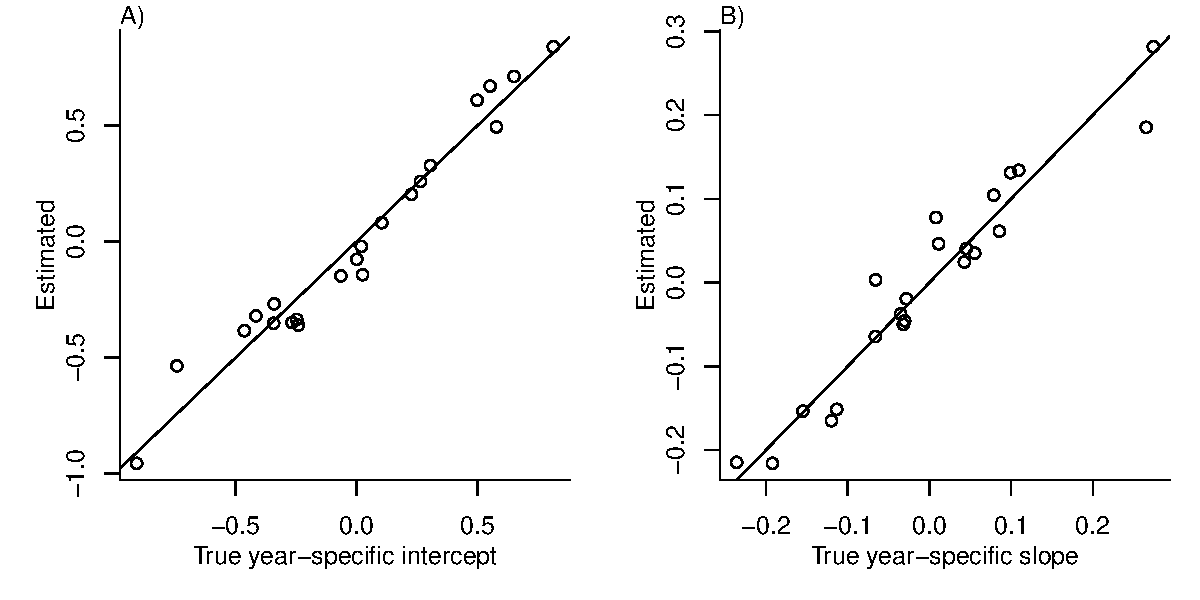
\includegraphics[width=\textwidth]{figures/SimpleShrinkage.pdf}}

  
\end{document}